% A list of all figure files:
% Those produced by TraubMemorial.m
%	f3plot.eps
%	f3foolplot.eps
%	sampling-funappxg.eps
%	sampling-funming.eps
%
% Produced by cf_chebfun.m 
%	chebfun_errors.eps
%
% Produced by traubpaper_funappx_g_test.m
%	traub_funappxNoPenalty_g_test.eps



\documentclass[review]{elsarticle}
%\documentclass[final]{elsarticle}

\usepackage{amsmath,amssymb,amsthm,xspace,mathtools,booktabs,hyperref,color}
\usepackage{mathrsfs,verbatim,xspace}

\allowdisplaybreaks
\newcommand{\bvec}[1]{\boldsymbol{#1}}
%\newcommand{\bvec}[1]{\text{\boldmath$#1$}}
\newcommand{\avec}[1]{\vec{#1}}
%\renewcommand{\vec}[1] {\text{\boldmath$#1$}}
%\renewcommand{\vec}[1]{\ensuremath{\mathbf{#1}}}
\newcommand{\vecsym}[1]{\ensuremath{\boldsymbol{#1}}}
\def\bbl{\text{\boldmath$\{$}}
\def\bbr{\text{\boldmath$\}$}}
\newcommand{\bbrace}[1]{\bbl #1 \bbr}
\newcommand{\bbbrace}[1]{\mathopen{\pmb{\bigg\{}}#1\mathclose{\pmb{\bigg\}}}}
%\def\bbl{\boldsymbol{\left \{}}
%\def\bbr{\boldsymbol{\right \}}}
\def\betahat{\hat\beta}
%\def\e{\text{e}}
%\def\E{\text{E}}
\newcommand{\dif}{{\rm d}}

\newlength{\overwdth}
\def\overstrike#1{ 
\settowidth{\overwdth}{#1}\makebox[0pt][l]{\rule[0.5ex]{\overwdth}{0.1ex}}#1}

\def\abs#1{\ensuremath{\left \lvert #1 \right \rvert}}
\newcommand{\bigabs}[1]{\ensuremath{\bigl \lvert #1 \bigr \rvert}}
\newcommand{\Bigabs}[1]{\ensuremath{\Bigl \lvert #1 \Bigr \rvert}}
\newcommand{\biggabs}[1]{\ensuremath{\biggl \lvert #1 \biggr \rvert}}
\newcommand{\Biggabs}[1]{\ensuremath{\Biggl \lvert #1 \Biggr \rvert}}
\newcommand{\norm}[2][{}]{\ensuremath{\left \lVert #2 \right \rVert}_{#1}}
\newcommand{\bignorm}[2][{}]{\ensuremath{\bigl \lVert #2 \bigr \rVert}_{#1}}
\newcommand{\Bignorm}[2][{}]{\ensuremath{\Bigl \lVert #2 \Bigr \rVert}_{#1}}
\newcommand{\biggnorm}[2][{}]{\ensuremath{\biggl \lVert #2 \biggr \rVert}_{#1}}
\newcommand{\ip}[3][{}]{\ensuremath{\left \langle #2, #3 \right \rangle_{#1}}}

\newcommand{\bigvecpar}[3]{\ensuremath{\bigl ( #1 \bigr )_{#2}^{#3}}}
\newcommand{\Bigvecpar}[3]{\ensuremath{\Bigl ( #1 \Bigr )_{#2}^{#3}}}
\newcommand{\biggvecpar}[3]{\ensuremath{\biggl ( #1 \biggr )_{#2}^{#3}}}
\newcommand{\bigpar}[1]{\ensuremath{\bigl ( #1 \bigr )}}
\newcommand{\Bigpar}[1]{\ensuremath{\Bigl ( #1 \Bigr )}}
\newcommand{\biggpar}[1]{\ensuremath{\biggl ( #1 \biggr )}}

\newcommand{\IIDsim}{\overset{\textup{IID}}{\sim}}

\DeclareMathOperator{\success}{succ}
\DeclareMathOperator{\sinc}{sinc}
\DeclareMathOperator{\sech}{sech}
\DeclareMathOperator{\csch}{csch}
\DeclareMathOperator{\dist}{dist}
\DeclareMathOperator{\spn}{span}
\DeclareMathOperator{\sgn}{sgn}
\DeclareMathOperator*{\rmse}{rmse}
\DeclareMathOperator{\Prob}{\mathbb{P}}
\DeclareMathOperator{\Ex}{\mathbb{E}}
\DeclareMathOperator{\rank}{rank}
\DeclareMathOperator{\erfc}{erfc}
\DeclareMathOperator{\erf}{erf}
\DeclareMathOperator{\cov}{cov}
\DeclareMathOperator{\cost}{cost}
\DeclareMathOperator{\comp}{comp}
\DeclareMathOperator{\corr}{corr}
\DeclareMathOperator{\diag}{diag}
\DeclareMathOperator{\var}{var}
\DeclareMathOperator{\opt}{opt}
\DeclareMathOperator{\brandnew}{new}
\DeclareMathOperator{\std}{std}
\DeclareMathOperator{\kurt}{kurt}
\DeclareMathOperator{\med}{med}
\DeclareMathOperator{\vol}{vol}
\DeclareMathOperator{\bias}{bias}
\DeclareMathOperator*{\argmin}{argmin}
\DeclareMathOperator{\sign}{sign}
\DeclareMathOperator{\spann}{span}
\DeclareMathOperator{\cond}{cond}
\DeclareMathOperator{\trace}{trace}
\DeclareMathOperator{\Si}{Si}
%\DeclareMathOperator{\diag}{diag}
\DeclareMathOperator{\col}{col}
\DeclareMathOperator{\nullspace}{null}
\DeclareMathOperator{\Order}{{\mathcal O}}
%\DeclareMathOperator{\rank}{rank}

\newcommand{\vzero}{\bvec{0}}
\newcommand{\vone}{\bvec{1}}
\newcommand{\vinf}{\bvec{\infty}}
\newcommand{\va}{\bvec{a}}
\newcommand{\vA}{\bvec{A}}
\newcommand{\vb}{\bvec{b}}
\newcommand{\vB}{\bvec{B}}
\newcommand{\vc}{\bvec{c}}
\newcommand{\vd}{\bvec{d}}
\newcommand{\vD}{\bvec{D}}
\newcommand{\ve}{\bvec{e}}
\newcommand{\vf}{\bvec{f}}
\newcommand{\vF}{\bvec{F}}
\newcommand{\vg}{\bvec{g}}
\newcommand{\vG}{\bvec{G}}
\newcommand{\vh}{\bvec{h}}
\newcommand{\vi}{\bvec{i}}
\newcommand{\vj}{\bvec{j}}
\newcommand{\vk}{\bvec{k}}
\newcommand{\vl}{\bvec{l}}
\newcommand{\vell}{\bvec{\ell}}
\newcommand{\vL}{\bvec{L}}
\newcommand{\vm}{\bvec{m}}
\newcommand{\vp}{\bvec{p}}
\newcommand{\vq}{\bvec{q}}
\newcommand{\vr}{\bvec{r}}
\newcommand{\vs}{\bvec{s}}
\newcommand{\vS}{\bvec{S}}
\newcommand{\vt}{\bvec{t}}
\newcommand{\vT}{\bvec{T}}
\newcommand{\vu}{\bvec{u}}
\newcommand{\vU}{\bvec{U}}
\newcommand{\vv}{\bvec{v}}
\newcommand{\vV}{\bvec{V}}
\newcommand{\vw}{\bvec{w}}
\newcommand{\vW}{\bvec{W}}
\newcommand{\vx}{\bvec{x}}
\newcommand{\vX}{\bvec{X}}
\newcommand{\vy}{\bvec{y}}
\newcommand{\vY}{\bvec{Y}}
\newcommand{\vz}{\bvec{z}}
\newcommand{\vZ}{\bvec{Z}}

\newcommand{\ai}{\avec{\imath}}
\newcommand{\ak}{\avec{k}}
\newcommand{\avi}{\avec{\bvec{\imath}}}
\newcommand{\at}{\avec{t}}
\newcommand{\avt}{\avec{\vt}}
\newcommand{\ax}{\avec{x}}
\newcommand{\ah}{\avec{h}}
\newcommand{\akappa}{\avec{\kappa}}
\newcommand{\avx}{\avec{\vx}}
\newcommand{\ay}{\avec{y}}
\newcommand{\avy}{\avec{\vy}}
\newcommand{\avz}{\avec{\vz}}
\newcommand{\avzero}{\avec{\vzero}}
\newcommand{\aomega}{\avec{\omega}}
\newcommand{\avomega}{\avec{\vomega}}
\newcommand{\anu}{\avec{\nu}}
\newcommand{\avnu}{\avec{\vnu}}
\newcommand{\aDelta}{\avec{\Delta}}
\newcommand{\avDelta}{\avec{\vDelta}}

\newcommand{\valpha}{\bvec{\alpha}}
\newcommand{\vbeta}{\bvec{\beta}}
\newcommand{\vgamma}{\bvec{\gamma}}
\newcommand{\vdelta}{\bvec{\delta}}
\newcommand{\vDelta}{\bvec{\Delta}}
\newcommand{\vphi}{\bvec{\phi}}
\newcommand{\vvphi}{\bvec{\varphi}}
\newcommand{\vomega}{\bvec{\omega}}
\newcommand{\vlambda}{\bvec{\lambda}}
\newcommand{\vmu}{\bvec{\mu}}
\newcommand{\vnu}{\bvec{\nu}}
\newcommand{\vpsi}{\bvec{\psi}}
\newcommand{\vepsilon}{\bvec{\epsilon}}
\newcommand{\veps}{\bvec{\varepsilon}}
\newcommand{\veta}{\bvec{\eta}}
\newcommand{\vxi}{\bvec{\xi}}
\newcommand{\vtheta}{\bvec{\theta}}
\newcommand{\vtau}{\bvec{\tau}}
\newcommand{\vzeta}{\bvec{\zeta}}

\newcommand{\hvb}{\hat{\vb}}
\newcommand{\hcc}{\widehat{\cc}}
\newcommand{\hD}{\widehat{D}}
\newcommand{\hE}{\widehat{E}}
\newcommand{\hf}{\widehat{f}}
\newcommand{\hF}{\widehat{F}}
\newcommand{\hg}{\hat{g}}
\newcommand{\hvf}{\widehat{\bvec{f}}}
\newcommand{\hh}{\hat{h}}
\newcommand{\hH}{\widehat{H}}
\newcommand{\hi}{\hat{\imath}}
\newcommand{\hI}{\hat{I}}
\newcommand{\hci}{\widehat{\ci}}
\newcommand{\hj}{\hat{\jmath}}
\newcommand{\hp}{\hat{p}}
\newcommand{\hP}{\hat{P}}
\newcommand{\hS}{\widehat{S}}
\newcommand{\hv}{\hat{v}}
\newcommand{\hV}{\widehat{V}}
\newcommand{\hx}{\hat{x}}
\newcommand{\hX}{\widehat{X}}
\newcommand{\hvX}{\widehat{\vX}}
\newcommand{\hy}{\hat{y}}
\newcommand{\hvy}{\hat{\vy}}
\newcommand{\hY}{\widehat{Y}}
\newcommand{\hvY}{\widehat{\vY}}
\newcommand{\hZ}{\widehat{Z}}
\newcommand{\hvZ}{\widehat{\vZ}}

\newcommand{\halpha}{\hat{\alpha}}
\newcommand{\hvalpha}{\hat{\valpha}}
\newcommand{\hbeta}{\hat{\beta}}
\newcommand{\hvbeta}{\hat{\vbeta}}
\newcommand{\hgamma}{\hat{\gamma}}
\newcommand{\hvgamma}{\hat{\vgamma}}
\newcommand{\hdelta}{\hat{\delta}}
\newcommand{\hvareps}{\hat{\varepsilon}}
\newcommand{\hveps}{\hat{\veps}}
\newcommand{\hmu}{\hat{\mu}}
\newcommand{\hnu}{\hat{\nu}}
\newcommand{\hvnu}{\widehat{\vnu}}
\newcommand{\homega}{\widehat{\omega}}
\newcommand{\hrho}{\hat{\rho}}
\newcommand{\hsigma}{\hat{\sigma}}
\newcommand{\htheta}{\hat{\theta}}
\newcommand{\hTheta}{\hat{\Theta}}
\newcommand{\htau}{\hat{\tau}}
\newcommand{\hxi}{\hat{\xi}}
\newcommand{\hvxi}{\hat{\vxi}}

\newcommand{\otau}{\overline{\tau}}
\newcommand{\oY}{\overline{Y}}

\newcommand{\rD}{\mathring{D}}
\newcommand{\rf}{\mathring{f}}
\newcommand{\rV}{\mathring{V}}

\newcommand{\ta}{\tilde{a}}
\newcommand{\tA}{\tilde{A}}
\newcommand{\tmA}{\widetilde{\mA}}
\newcommand{\tvb}{\tilde{\vb}}
\newcommand{\tcb}{\widetilde{\cb}}
\newcommand{\tB}{\widetilde{B}}
\newcommand{\tc}{\tilde{c}}
\newcommand{\tvc}{\tilde{\vc}}
\newcommand{\tfc}{\tilde{\fc}}
\newcommand{\tC}{\widetilde{C}}
\newcommand{\tcc}{\widetilde{\cc}}
\newcommand{\tD}{\widetilde{D}}
\newcommand{\te}{\tilde{e}}
\newcommand{\tE}{\widetilde{E}}
\newcommand{\tf}{\widetilde{f}}
\newcommand{\tF}{\widetilde{F}}
\newcommand{\tvf}{\tilde{\vf}}
\newcommand{\tcf}{\widetilde{\cf}}
\newcommand{\tg}{\tilde{g}}
\newcommand{\tG}{\widetilde{G}}
\newcommand{\tildeh}{\tilde{h}}
\newcommand{\tH}{\widetilde{H}}
\newcommand{\tch}{\widetilde{\ch}}
\newcommand{\tK}{\widetilde{K}}
\newcommand{\tvk}{\tilde{\vk}}
\newcommand{\tM}{\widetilde{M}}
\newcommand{\tn}{\tilde{n}}
\newcommand{\tN}{\widetilde{N}}
\newcommand{\tQ}{\widetilde{Q}}
\newcommand{\tR}{\widetilde{R}}
\newcommand{\tS}{\widetilde{S}}
\newcommand{\tvS}{\widetilde{\vS}}
\newcommand{\tT}{\widetilde{T}}
\newcommand{\tv}{\tilde{v}}
\newcommand{\tV}{\widetilde{V}}
\newcommand{\tvx}{\tilde{\vx}}
\newcommand{\tW}{\widetilde{W}}
\newcommand{\tx}{\tilde{x}}
\newcommand{\tX}{\widetilde{X}}
\newcommand{\tvX}{\widetilde{\vX}}
\newcommand{\ty}{\tilde{y}}
\newcommand{\tvy}{\tilde{\vy}}
\newcommand{\tz}{\tilde{z}}
\newcommand{\tZ}{\widetilde{Z}}
\newcommand{\tL}{\tilde{L}}
\newcommand{\tP}{\widetilde{P}}
\newcommand{\tY}{\widetilde{Y}}
\newcommand{\tmH}{\widetilde{\mH}}
\newcommand{\tmK}{\widetilde{\mK}}
\newcommand{\tmM}{\widetilde{\mM}}
\newcommand{\tmQ}{\widetilde{\mQ}}
\newcommand{\tct}{\widetilde{\ct}}
\newcommand{\talpha}{\tilde{\alpha}}
\newcommand{\tdelta}{\tilde{\delta}}
\newcommand{\tDelta}{\tilde{\Delta}}
\newcommand{\tvareps}{\tilde{\varepsilon}}
\newcommand{\tveps}{\tilde{\veps}}
\newcommand{\tlambda}{\tilde{\lambda}}
\newcommand{\tmu}{\tilde{\mu}}
\newcommand{\tnu}{\tilde{\nu}}
\newcommand{\trho}{\tilde{\rho}}
\newcommand{\tvarrho}{\tilde{\varrho}}
\newcommand{\ttheta}{\tilde{\theta}}
\newcommand{\tsigma}{\tilde{\sigma}}
\newcommand{\tvmu}{\tilde{\vmu}}
\newcommand{\tphi}{\tilde{\phi}}
\newcommand{\tPhi}{\widetilde{\Phi}}
\newcommand{\tvphi}{\tilde{\vphi}}
\newcommand{\ttau}{\tilde{\tau}}
\newcommand{\txi}{\tilde{\xi}}
\newcommand{\tvxi}{\tilde{\vxi}}


\newcommand{\mA}{\mathsf{A}}
\newcommand{\mB}{\mathsf{B}}
\newcommand{\mC}{\mathsf{C}}
\newcommand{\vmC}{\bvec{\mC}}
\newcommand{\mD}{\mathsf{D}}
\newcommand{\mF}{\mathsf{F}}
\newcommand{\mG}{\mathsf{G}}
\newcommand{\mH}{\mathsf{H}}
\newcommand{\mI}{\mathsf{I}}
\newcommand{\mK}{\mathsf{K}}
\newcommand{\mL}{\mathsf{L}}
\newcommand{\mM}{\mathsf{M}}
\newcommand{\mP}{\mathsf{P}}
\newcommand{\mQ}{\mathsf{Q}}
\newcommand{\mR}{\mathsf{R}}
\newcommand{\mS}{\mathsf{S}}
\newcommand{\mT}{\mathsf{T}}
\newcommand{\mU}{\mathsf{U}}
\newcommand{\mV}{\mathsf{V}}
\newcommand{\mW}{\mathsf{W}}
\newcommand{\mX}{\mathsf{X}}
\newcommand{\mLambda}{\mathsf{\Lambda}}
\newcommand{\mSigma}{\mathsf{\Sigma}}
\newcommand{\mzero}{\mathsf{0}}
\newcommand{\mGamma}{\mathsf{\Gamma}}

\newcommand{\bbE}{\mathbb{E}}
\newcommand{\bbF}{\mathbb{F}}
\newcommand{\bbK}{\mathbb{K}}
\newcommand{\bbZ}{\mathbb{Z}}
\newcommand{\bbone}{\mathbbm{1}}
\newcommand{\naturals}{\mathbb{N}}
\newcommand{\reals}{\mathbb{R}}
\newcommand{\integers}{\mathbb{Z}}
\newcommand{\natzero}{\mathbb{N}_{0}}
\newcommand{\rationals}{\mathbb{Q}}
\newcommand{\complex}{\mathbb{C}}

\newcommand{\ca}{\mathcal{A}}
\newcommand{\cb}{\mathcal{B}}
\providecommand{\cc}{\mathcal{C}}
\newcommand{\cd}{\mathcal{D}}
\newcommand{\cf}{\mathcal{F}}
\newcommand{\cg}{\mathcal{G}}
\newcommand{\ch}{\mathcal{H}}
\newcommand{\ci}{\mathcal{I}}
\newcommand{\cj}{\mathcal{J}}
\newcommand{\ck}{\mathcal{K}}
\newcommand{\cl}{\mathcal{L}}
\newcommand{\cm}{\mathcal{M}}
\newcommand{\tcm}{\widetilde{\cm}}
\newcommand{\cn}{\mathcal{N}}
\newcommand{\cp}{\mathcal{P}}
\newcommand{\calr}{\mathcal{R}}
\newcommand{\cs}{\mathcal{S}}
\newcommand{\ct}{\mathcal{T}}
\newcommand{\cu}{\mathcal{U}}
\newcommand{\cv}{\mathcal{V}}
\newcommand{\cw}{\mathcal{W}}
\newcommand{\cx}{\mathcal{X}}
\newcommand{\tcx}{\widetilde{\cx}}
\newcommand{\cy}{\mathcal{Y}}
\newcommand{\cz}{\mathcal{Z}}

\newcommand{\fc}{\mathfrak{c}}
\newcommand{\fC}{\mathfrak{C}}
\newcommand{\fh}{\mathfrak{h}}
\newcommand{\fu}{\mathfrak{u}}

\newcommand{\me}{\ensuremath{\mathrm{e}}} % for math number 'e', 2.718 281 8..., tha base of natural logarithms
\newcommand{\mi}{\ensuremath{\mathrm{i}}} % for math number 'i', the imaginary unit
\newcommand{\mpi}{\ensuremath{\mathrm{\pi}}} % for math number 'pi', the circumference of a circle of diameter 1


\journal{Journal of Complexity}

%%%%%%%%%%%%%%%%%%%%%%%
%% Elsevier bibliography styles
%%%%%%%%%%%%%%%%%%%%%%%
%% To change the style, put a % in front of the second line of the current style and
%% remove the % from the second line of the style you would like to use.
%%%%%%%%%%%%%%%%%%%%%%%

%% Numbered
\bibliographystyle{model1-num-names}

%% Numbered without titles
%\bibliographystyle{model1a-num-names}

%% Harvard
%\bibliographystyle{model2-names.bst}\biboptions{authoryear}

%% Vancouver numbered
%\usepackage{numcompress}\bibliographystyle{model3-num-names}

%% Vancouver name/year
%\usepackage{numcompress} \bibliographystyle{model4-names}\biboptions{authoryear}

%% APA style
%\bibliographystyle{model5-names}\biboptions{authoryear}

%% AMA style
%\usepackage{numcompress}\bibliographystyle{model6-num-names}

%% `Elsevier LaTeX' style
%\bibliographystyle{elsarticle-num}
%%%%%%%%%%%%%%%%%%%%%%%

\newcommand{\abstol}{\varepsilon}
\newcommand{\zton}{0\!:\!n}
\newcommand{\oton}{1\!:\!n}
\newcommand{\datasites}{x_{0:n}}
\makeatletter
\newcommand{\vast}{\bBigg@{4}}
\newcommand{\Vast}{\bBigg@{6}}
\makeatother
%\newdefinition{algo}{Algorithm}
\theoremstyle{definition}
\newtheorem*{algoA}{Algorithm $A$}
\newtheorem*{algoM}{Algorithm $M$}

\newcommand{\vastl}{\mathopen\vast}
\newcommand{\vastm}{\mathrel\vast}
\newcommand{\vastr}{\mathclose\vast}
\newcommand{\Vastl}{\mathopen\Vast}
\newcommand{\Vastm}{\mathrel\Vast}
\newcommand{\Vastr}{\mathclose\Vast}
\renewcommand{\cw}{W}

\definecolor{orange}{rgb}{1.0,0.3,0.0}
\definecolor{violet}{rgb}{0.75,0,1}
\definecolor{darkgreen}{rgb}{0,0.6,0}
\newcommand{\frednote}[1]{  {\textcolor{red}  {\mbox{**Fred:} #1}}}
\newcommand{\yuhannote}[1]{  {\textcolor{darkgreen}  {\mbox{**Yuhan:} #1}}}
\newcommand{\xinnote}[1]{ {\textcolor{violet}  {\mbox{**Xin:} #1}}}
\newcommand{\scnote}[1]{ {\textcolor{orange}  {\mbox{**SC:} #1}}}

\newcommand{\Ixl}{I_{x,l}}
\newcommand{\Ixlx}{I_{x,\ell(x)}}
\newcommand{\Ixrlx}{I_{x,\rell(x)}}
\newcommand{\Ixhlx}{I_{x,\hell(x)}}
\newcommand{\hell}{\hat{\ell}}
\newcommand{\tell}{\tilde{\ell}}
\newcommand{\ttL}{\widetilde{\widetilde{L}}}
\newcommand{\chL}{\widehat{L}}
\newcommand{\rell}{\mathring{\ell}}
\newcommand{\tgamma}{\widetilde{\gamma}}
\newcommand{\hM}{\widehat{M}}
\DeclareMathOperator{\lo}{lo}
\DeclareMathOperator{\ninit}{ninit}
\DeclareMathOperator{\errest}{errest}
\DeclareMathOperator{\oerr}{\overline{err}}
\DeclareMathOperator{\herr}{\widehat{err}}
\newtheorem{theorem}{Theorem}
\newtheorem{exmp}{Example}
\newtheorem{prop}[theorem]{Proposition}
\newcommand{\funappxg}{\texttt{funappx\_g}\xspace}
\newcommand{\funappxglobalg}{\texttt{funappxglobal\_g}\xspace}
\newcommand{\funming}{\texttt{funmin\_g}\xspace}
\newcommand{\fminbnd}{\texttt{fminbnd}\xspace}
\newcommand{\integralg}{\texttt{integral\_g}\xspace}
\newcommand{\cosappx}{\widehat{\operatorname*{cos}}}
\newcommand{\sinappx}{\widehat{\operatorname*{sin}}}
\newcommand{\minfi}{\min\limits_{i \in 0:n} f(x_i)} %minf(xi)
\newcommand{\minfii}{\min(f(x_{i-1}), f(x_i))} %min{f(x_i-1),f(x_i)}
\begin{document}

\begin{frontmatter}

\title{Local Adaption for Approximation and Minimization of Univariate Functions}


%% Group authors per affiliation:
\author{Sou-Cheng T.~Choi}
\author{Yuhan Ding}
\author{Fred J.~Hickernell}
\address{Department of Applied Mathematics, Illinois Institute of Technology, 
%RE 208, 10 West 32$^{\text{nd}}$ Street, Chicago, Illinois, 60616, 
USA}
\author{Xin Tong}
\address{Department of Mathematics, Statistics, and Computer Science, University of Illinois at Chicago, % Room 322 SEO, 851 S. Morgan Street, Chicago, Illinois, 60607, 
USA}



\begin{abstract}
Most commonly used \emph{adaptive} algorithms for function approximation and global
minimization lack theoretical guarantees. Our new locally adaptive algorithms
are guaranteed to provide approximants that satisfy a user-specified absolute
error tolerance for a cone, $\cc$, of non-spiky functions in the Sobolev space
$\cw^{2,\infty}$. Our algorithms automatically determine where to sample the
function---sampling more densely where the second derivative is larger. The
computational cost of our algorithm for approximating a univariate function $f$ on a
bounded interval with $L^{\infty}$-error no greater than $\abstol$ is
$\smash{\Order\Bigl(\sqrt{\norm[\frac12]{f''}/\abstol}\Bigr)}$, the
same order as that of the best function approximation algorithm for functions in
$\cc$. The computational cost of our global minimization algorithm is of the same order 
and can cost substantially less if $f$
significantly exceeds its minimum over much of its domain. Our
algorithms have been implemented in our Guaranteed Automatic Integration
Library. Numerical examples are presented to illustrate the performance of our
algorithms.
\end{abstract}

\begin{keyword}
adaption \sep automatic \sep computational complexity \sep function approximation 
\sep function recovery \sep minimization \sep optimization
\MSC[2010]  65D05 \sep 65D07 \sep 65K05 \sep 68Q25
\end{keyword}

\end{frontmatter}

%%%%%%%%%%%%%%%%%%%%%%%%%%%%%%%%%%%%%%%%%%%%%%%%%%
\section{Introduction} \label{sec:intro}
%%%%%%%%%%%%%%%%%%%%%%%%%%%%%%%%%%%%%%%%%%%%%%%%%%

Our goal is to solve univariate function approximation and global minimization
problems by adaptive algorithms. For some suitable set, $\cc$, of continuously
differentiable, real-valued functions defined on a finite interval $[a,b]$, we
construct algorithms $A:(\cc,(0,\infty)) \to L^{\infty}[a,b]$ and $M:
(\cc,(0,\infty)) \to \reals$ such that for any $f \in \cc$ and any error
tolerance $\abstol > 0$, \begin{gather} \norm{f - A(f,\abstol)} \le \abstol,
\tag{APP} \label{appxprob} \\ 0 \le M(f,\abstol) - \min_{a \le x \le b} f(x) \le
\abstol. \tag{MIN} \label{optprob} \end{gather} Here, $\norm{\cdot}$ denotes the
$L^{\infty}$-norm on $[a,b]$. The algorithms $A$ and $M$ depend only on function
values.

These algorithms proceed iteratively until their data-dependent stopping
criteria are satisfied. The input functions are sampled sample nonuniformly over
the interval $[a,b]$, with the sampling density determined by the function data.
We call our algorithms \emph{locally adaptive}, to distinguish them from
globally adaptive algorithms that have a fixed sampling pattern and only the
sample size determined adaptively.

%---------------------------------------------------------------
\subsection{Key Ideas in Our Algorithms} \label{subsec:keyideas}
%---------------------------------------------------------------

Our algorithms $A$ and $M$ are based on a \emph{linear spline}: 
\begin{multline} \label{splinedef}
   S(f,\datasites)(x) =  
   \frac{x-x_i}{x_{i-1} - x_i} f(x_{i-1}) + \frac{x-x_{i-1}}{x_{i} - x_{i-1}}f(x_i), 
\\ x_{i-1} \le x \le x_i, \quad i \in \oton.
\end{multline}
Here ${0\!:\!n}$ is shorthand for ${0, \ldots, n}$, and $\datasites$ is an
ordered sequence of $n+1$ points that includes the endpoints of the interval,
i.e., $a=:x_0 <x_1 < \cdots < x_{n-1} < x_{n}:=b$. We call such a sequence a
\emph{partition} of $[a,b]$. The error of the linear spline is bounded in terms
of the second derivative of the input function as follows \cite[Theorem
3.3]{BurFaiBur16a}:
\begin{equation} \label{appxerrbda}
	\norm[{[x_{i-1},x_i]}]{f - S(f,\datasites)} 
	\le \frac{(x_i - x_{i-1})^2\norm[{[x_{i-1},x_i]}]{f''}}{8}, 
\end{equation}
where $\norm[{[\alpha,\beta]}]{f}$ denotes the norm of $f$ restricted to the
interval $[\alpha,\beta] \subset [a,b]$. This error bound leads us to focus on
input functions in the Sobolev space $\cw^{2,\infty} := \{f \in C^1[a,b] :
\norm{f''} < \infty \}$.

Algorithms $A$ and $M$ require an upper bound on $\norm[{[x_{i-1},x_i]}]{f''}$
to make use of~\eqref{appxerrbda}. A nonadpative algorithm might assume that
$\norm{f''} \le \sigma$, for some known~$\sigma$, and proceed to choose $n =
\bigl \lceil (b-a)\smash{\sqrt{\sigma/(8 \varepsilon)}} \, \bigr \rceil$, $x_i = a +
i(b-a)/n$, $i \in 0\!:\!n$. However, providing an upper bound on $\norm{f''}$ is
often impractical, and so we propose adaptive algorithms that do not
require such information.

However, one must have some a priori information about $f \in \cw^{2,\infty} $
to construct successful algorithms for \eqref{appxprob} or \eqref{optprob}.
Suppose that algorithm $A$ satisfies \eqref{appxprob} for the zero function, and
$A(0,\varepsilon)$ uses the data sites $x_{0:n}\subset [a,b]$. Then one can
construct a \emph{nonzero} function $f \in \cw^{2,\infty}$ satisfying $f(x_i) =
0$, $i\in \zton$ but with $\norm{f - A(f,\abstol)} = \norm{f -
A(0,\abstol)} > \varepsilon$.

Our set $\cc \subset \cw^{2,\infty}$ for which $A$ and $M$ succeed is chosen to
include only those functions whose second derivatives do not change dramatically
over a short distance. The precise definition is given in Section
\ref{sec:cone}. This allows us to use second-order divided differences to
construct rigorous upper bounds on the linear spline error in
\eqref{appxerrbda}. These data-driven error bounds inform the stopping criteria
for Algorithm $A$ in Section \ref{subsec:appxalgo} and Algorithm $M$ in Section
\ref{sec:minalgo}.

The computational cost of Algorithm $A$ is analyzed in Section
\ref{subsec:appxcost} and is shown to be
$\smash{\Order\Bigl(\sqrt{\norm[\frac12]{f''}/\abstol}\Bigr)}$ as $\abstol \to 0$. Here,
$\norm[\frac12]{\cdot}$ denotes the $L^{\frac12}$-quasi-norm: $\norm[p]{f} :=
\bigl(\int_a^b \abs{f}^p \, \dif x \bigr)^{1/p}$, $0 < p < \infty$. Since
$\norm[\frac12]{f''}$ can be much smaller than $\norm{f''}$, locally adaptive
algorithms can be more efficient than globally adaptive algorithms, whose
computational costs are proportional to $\sqrt{\norm{f''}/\abstol}$. The
computational complexity of \eqref{appxprob} is determined in Section
\ref{subsec:appxcomp} to be
$\Order\Bigl(\smash{\sqrt{\norm[\frac12]{f''}/\abstol}}\Bigr)$ as well.

The computational cost of the optimization algorithm $M$ is analyzed in
Section~\ref{subsec:optcost}. A lower bound on the computational complexity of
\eqref{optprob} is a subject for future investigation.

Our algorithms are implemented in our MATLAB Guaranteed Automatic
Integration Library (GAIL) \cite{ChoEtal15a}. Section \ref{sec:examples}
provides numerical examples of our algorithms and compares their
performances with MATLAB's and Chebfun's algorithms. We note cases where our
algorithms are successful in meeting the error tolerance, and the other
algorithms are not.

%---------------------------------------------------------------
\subsection{Related Work on Adaptive Algorithms}
%---------------------------------------------------------------

Adaptive algorithms relieve the user of having to specify the number of samples
required. Only the desired error tolerance is needed. Existing adaptive
numerical algorithms for function approximation, such as the MATLAB toolbox
Chebfun \citep{TrefEtal16a}, suceed for some $f$, but fail for other $f$. No
theory explains for which $f$ Chebfun succeeds. A corresponding situation exists
for minimization algorithms, such as \texttt{min} in Chebfun or MATLAB's
built-in \texttt{fminbnd} \citep{MAT9.0}.

Our theoretically justified Algorithms $A$ and $M$ build upon the ideas used to
construct the adaptive algorithms in \cite{HicEtal14b, Din15a, HicEtal14a,
HicJim16a, Jia16a, JimHic16a,Ton14a}. Like here, in all those previous cases, a
cone, $\cc$, of input functions is identified for which the adaptive algorithms
succeed. However, unlike the algorithms in \cite{HicEtal14b, Din15a,
HicEtal14a,Ton14a}, the cone here does not appeal to a weaker norm. Also, unlike
the globally adaptive approximation and optimization algorithms in
\cite{HicEtal14b,Ton14a}, the algorithms proposed here are locally adaptive,
sampling the interval non-uniformly.

Novak \cite{Nov96a} summarizes the settings under which adaption may provide an
advantage over nonadaption. For linear problems, such as~\eqref{appxprob},
adaption has no advantage if the set of functions being considered is symmetric
and convex \cite[Theorem 1]{Nov96a}, \cite[Chapter 4, Theorem
5.2.1]{TraWasWoz88}. The cone $\cc$ defined for our approximation problem
\eqref{appxprob} is symmetric, but not convex. Plaskota et al.~\cite{PlaEtal08a}
have developed adaptive algorithms for functions with singularities. Our
algorithms are not designed for such functions. Rather they are
designed to be efficient when the second derivative is large in a small part of
the domain.

Plaskota \cite{Pla15a} has developed an adaptive Simpson's algorithm for
approximating $\int_a^b f(x) \, \dif x$ assuming that $f^{(4)}(x) \ge 0$ for all
$x \in [a,b]$. His algorithm relies on divided differences, like ours do. His
error is asymptotically proportional to $\norm[\frac14]{f^{(4)}}$, which is
analogous to the $\norm[\frac12]{f''}$ that appears in our analysis.

There is a significant literature on theoretically justified algorithms based on
interval arithmetic \cite{MoKeCl09, Rum10a}, which are implemented in
INTLAB~\cite{Rum99a}. This approach assumes that functions have interval inputs
and outputs. We focus on the more common situation where functions have point
inputs and outputs.

%%%%%%%%%%%%%%%%%%%%%%%%%%%%%%%%%%%%%%%%%%%%%%%%%%
\section{The Cone, $\cc$, of Functions of Interest} \label{sec:cone}
%%%%%%%%%%%%%%%%%%%%%%%%%%%%%%%%%%%%%%%%%%%%%%%%%%

Linear splines \eqref{splinedef} are the foundation for adaptive algorithms $A$
and $M$. To bound the error of the linear spline in \eqref{appxerrbda}, our
algorithms construct data-based upper bounds on $\norm[{[\alpha, \beta]}]{f''}$
in terms of divided differences. For these bounds to hold, we must assume that
$f''(x)$ does not change drastically with respect to a small change in $x$.
These assumptions define our cone of functions, $\cc$, for which our algorithms
ultimately apply.

Let $p$ denote the Lagrange quadratic interpolating polynomial at the nodes
$\{\alpha, (\alpha + \beta)/2, \beta\}$, which may be written as
\begin{align}
\nonumber
   p(x) & := f(\alpha) + \frac{(x-\alpha)[f(\beta) - f(\alpha)]}{\beta - \alpha}  + (x-\alpha)(x-\beta) D(f,\alpha,\beta), 
\\ D(f,\alpha,\beta) &:= \frac{2[f(\beta) - 2f((\alpha + \beta)/2)) + f(\alpha)]}{(\beta - \alpha)^2}. \label{divdiffdef}
\end{align}
For any $f \in \cw^{2,\infty}$, the function $f - p$ has at least three distinct
zeros on $[\alpha,\beta]$, so $f' - p'$ has at least two distinct zeros on
$(\alpha,\beta)$, i.e., there exists $\xi_\pm$ with $\alpha < \xi_- < (\alpha +
\beta)/2 < \xi_+ < \beta$ with $f'(\xi_\pm) - p'(\xi_{\pm}) = 0$. Thus,
\begin{align} \label{NDDbdm}
     \norm[-\infty,{[\alpha,\beta]}]{f''} 
   & := \inf_{\alpha \le \eta < \zeta \le \beta} \abs{\frac{f'(\zeta) - f'(\eta)}{\zeta - \eta}} \nonumber
\\ & \le \abs{\frac{f'(\xi_+) - f'(\xi_-)}{\xi_+ - \xi_-}} 
   = \abs{\frac{p'(\xi_+) - p'(\xi_-)}{\xi_+ - \xi_-}} = 2 \abs{D(f,\alpha,\beta)}  \nonumber
\\ & \le \sup_{\alpha \le \eta < \zeta \le \beta} \abs{\frac{f'(\zeta) - f'(\eta)}{\zeta - \eta}} =: \norm[{[\alpha,\beta]}]{f''}.
\end{align}
This inequality tells us that twice the divided difference,
$2\abs{D(f,\alpha,\beta)}$, is a \emph{lower} bound for
$\norm[{[\alpha,\beta]}]{f''}$, which by itself is not helpful. But,
$2\abs{D(f,\alpha,\beta)}$, is an \emph{upper} bound for
$\norm[-\infty,{[\alpha,\beta]}]{f''}$. The cone of interesting functions,
$\cc$, will contain those $f$ for which $\norm[{[\alpha,\beta]}]{f''}$ is not
drastically different than the maximum of $\norm[-\infty,{[\beta - h_-,
\alpha]}]{f''}$ and $\norm[-\infty,{[\beta, \alpha+ h_+]}]{f''}$.

The cone $\cc$ is defined in terms of two numbers: an integer $n_{\ninit} \ge 5$
and a positive number $\fC_0 \ge 1$. Let
\begin{equation}
\label{hCdef}
\fh := \frac{3(b-a)}{n_{\ninit}-1}, \qquad \fC(h) := \frac{\fC_0 \fh}{\fh - h} \mbox{\, for \,} 0<h<\fh.
\end{equation}
For any $[\alpha, \beta] \subseteq [a,b]$ and any $h_{\pm}$ satisfying $0 <
\beta - \alpha < h_{\pm} < \fh$, define
\begin{equation} \label{tbdef}
B(f,\alpha,\beta,h_-,h_+) :=
\begin{cases}
   \max\bigl(\fC(h_{-}) \norm[-\infty,{[\beta-h_-,\alpha]}]{f},\fC(h_{+}) \norm[-\infty,{[\beta, \alpha+h_+]}]{f}\bigr), 
\\                                             \hspace{26ex} a \le \beta- h_- <  \alpha + h_+ \le b,
\\ \fC(h_{-}) \norm[-\infty,{[\beta-h_-,\alpha]}]{f},  \quad a \le \beta- h_- < b< \alpha + h_+,
\\ \fC(h_{+}) \norm[-\infty,{[\beta, \alpha+h_+]}]{f}, \quad \beta- h_- <  a  < \alpha + h_+ \le b.
\end{cases} 
\end{equation}
\begin{multline} \label{conedef}
 \cc := \Bigl \{
 f  \in    \cw^{2,\infty}:   \norm[{[\alpha,\beta]}]{f''}  \le B(f,\alpha,\beta,h_-,h_+)  \text{ for all } [\alpha,\beta] \subset [a,b],
\\ \text{and } 0 < \beta - \alpha < \max(h_{\pm}) < \fh  \Bigr \}.
\end{multline}
The set $\cc$ is a cone because $f \in \cc \implies cf \in \cc$ for all real
$c$. The integer $n_{\ninit}$ is the initial number of subintervals in
Algorithms $A$ and $M$. The parameter $\fC_0$ represents an upper bound on
$\norm[{[\alpha,\beta]}]{f''}/\norm[-\infty,{[\alpha,\beta]}]{f''}$ as $\beta -
\alpha \to 0$. Increasing either $n_{\ninit}$ or $\fC_0$ expands the cone to
include more functions.

We give an example of a parameterized family of functions whose members lie
inside $\cc$ if they are not too spiky.
%Consider the following two functions defined on $[-1,1]$ whose
%second derivatives oscillate wildly near $0$:
%\begin{gather*}
%f_1(x) = x^4 \sin(1/x), \\
% f_1''(x) =  (12x^2 - 1) \sin(1/x) -6 x \cos(1/x), \qquad x \ne 0 \\
%f_2(x) = 10  x^2 + f_1(x), \qquad f_2''(x) = 20+ f_1''(x).
%\end{gather*}
%These functions are plotted in Figure~\ref{f1f2fig}. Because $\norm[-\infty,{[\alpha,\beta]}]{f''_1} = 0 < 1 \le \norm[{[\alpha,\beta]}]{f''_1}$ for $-1 \le \alpha < 0 < \beta \le 1$,  $f_1$ cannot lie inside
%$\cc$ no matter how $n_{\ninit}$ and $\fC_0$ are chosen.   On the other hand,
%$\norm[{[\alpha,\beta]}]{f''_1} \le 27  \le 2 \norm[-\infty,{[\alpha,\beta]}]{f''_1}$ for all $-1 \le \alpha < \beta \le 1$,  so $f_2 \in
%\cc$ if $\fC_0 \ge 2$.
%
%\begin{figure}[t]
%\centering
%\includegraphics[width=5.6cm]{figure/f1f2plot.eps} \quad
%\includegraphics[width=5.9cm]{figure/f1closeplot.eps} \\
%\includegraphics[width=5.6cm]{figure/f1ppf2ppplot.eps} \quad
%\includegraphics[width=5.9cm]{figure/f2closeplot.eps}
%\caption{The examples $f_1$ and $f_2$ and their second derivatives. Note that
%$f_2''(x) = f_1''(x) + 20$. This figure is reproducible by {\tt TraubMemorial.m}
%in GAIL.}
%\label{f1f2fig}
%\end{figure}
Consider the following hump-shaped function defined on $[-1,1]$, whose
second derivative has jump discontinuities:
\begin{align} \label{f3def}
f_1(x) & = \begin{cases} \displaystyle
   \frac{1}{2\delta^2} \Bigl [4 \delta^2 + (x-c)^2 + (x-c-\delta)\abs{x-c-\delta}
\\ \qquad \qquad
    - (x-c+\delta)\abs{x-c+\delta} \Bigr ], & \abs{x-c} \le 2\delta,
\\ 0, & \text{otherwise},
\end{cases} 
\\ \nonumber
f''_1(x) & =
\begin{cases} \displaystyle
    \frac{1}{\delta^2} [1 + \sign(x-c-\delta) - \sign(x-c+\delta), & \abs{x-c} \le 2\delta,
\\ 0, & \text{otherwise}.
\end{cases}
\end{align}
Here $c$ and $\delta$ are parameters satisfying $-1 \le c-2 \delta < c+ 2\delta
\le 1$. This function and its second derivative are shown in Figure~\ref{f3fig}(a)
for $-c=\delta = 0.2$.


\begin{figure}[tb]
\centering
\begin{tabular}{cc}
\includegraphics[width=5.7cm]{figure/f3plot.eps}  
%\includegraphics[width=5.7cm]{figure/f3ppplot.eps}
& \includegraphics[width=5.7cm]{figure/f3foolplot.eps}
\\[1ex] (a) & (b)
\end{tabular}
\caption{(a) The example $f_1$ with $-c=\delta = 0.2$ and its piecewise constant
second derivative. %This figure is reproducible by {\tt TraubMemorial.m} in GAIL. 
(b) The fooling functions $\pm f_1$ used to prove~\eqref{lowbdW}. The case
$n=15$ is shown.  
This figure is reproducible by {\tt TraubMemorial.m} in GAIL.}
\label{f3fig}
\end{figure}



If the hump is wide enough, i.e., $\delta \ge 2 \fh$, then $f_1 \in \cc$ for any
choice of $\fC_0 \ge 1$. For for any $[\alpha,\beta]\subseteq [-1,1]$ and
$h_{\pm}$ satisfying the conditions in the definition of~$\cc$ in~\eqref{conedef}, 
it follows that
\begin{align*}
    & \norm{f''_1} = \delta^{-2} =
\begin{cases}
\norm[-\infty,{[\beta,\alpha+h_+]}]{f''_1}  %= \delta^{-2} = \norm{f''_1}
   & \text{if } \alpha\text{ or } \beta \in [c - 2\delta,  c - 1.5\delta]  
\\ & \qquad\quad \cup [c - \delta,  c + 0.5\delta] \cup [c + \delta, c+1.5\delta],
\\ \norm[-\infty,{[\beta - h_-,\alpha]}]{f''_1} %= \delta^{-2} = \norm{f''_1}
   & \text{if } \alpha\text{ or } \beta \in [c - 1.5\delta,  c - \delta]
\\ & \qquad\quad  \cup [c - 0.5 \delta,  c + \delta] \cup [c + 1.5\delta, c+2\delta].
\end{cases}
\end{align*}
Thus, $B(f,\alpha,\beta,h_-,h_+)\ge\norm[{[\alpha,\beta]}]{f''_1}$ for $\beta
\ge c - 2\delta$ or $\alpha \le c + 2\delta$. For $[\alpha,\beta] \subset [-1,c
- \delta) \cup (c+\delta, 1]$, it follows that $\norm[{[\alpha,\beta]}]{f''_1} =
0$, so $B(f,\alpha,\beta,h_-,h_+)\ge\norm[{[\alpha,\beta]}]{f''_1}$
automatically. Thus, the definition of the cone is satisfied.

However, if the hump is too narrow, i.e., $\delta < 2 \fh$, the function $f_1$
is too spiky to lie in the cone $\cc$ regardless of how $\fC_0$ is defined. For
$\alpha$, $\beta$, and $h$ satisfying
\[
0 < c - 3\alpha/2 -\alpha =  \beta - c+ 3\delta/2 < \delta/2 < c-3\delta/2 - \beta + h < \fh,
\]
it follows that for $h < \fh$,
\begin{gather*}
   \beta -  h < c - 2 \delta < \alpha < c - 3\alpha/2 < \beta < c - \delta < \alpha + h, 
\\ \norm[-\infty,{[\beta - h,\alpha]}]{f''_1} =\norm[-\infty,{[\beta,\alpha+h]}]{f''_1}=0 < \delta^{-2} =\norm[{[\alpha,\beta]}]{f''_1}.
\end{gather*}
This violates the definition of $\cc$. This example illustrates how the choice
of $\fh$ influences the width of a spiky function and determines whether it lies in
$\cc$.


%%%%%%%%%%%%%%%%%%%%%%%%%%%%%%%%%%%%%%%%%%%%%%%%%%
\section{The Function Approximation Algorithm, $A$}\label{sec:fappx}
%%%%%%%%%%%%%%%%%%%%%%%%%%%%%%%%%%%%%%%%%%%%%%%%%%

%---------------------------------------------------------------
\subsection{Algorithm $A$} \label{subsec:appxalgo}
%---------------------------------------------------------------

The idea of Algorithm $A$ is to use divided differences to provide upper bounds
on $\norm[-\infty,{[\beta - h_-, \alpha]}]{f}$ and $\norm[-\infty{[\beta,
\alpha+h_+]}]{f}$ via \eqref{NDDbdm}, which then provide an upper bound on
$\norm[{[\alpha,\beta]}]{f}$ via the definition of the cone, $\cc$, in
\eqref{conedef}. This in turn yields an upper bound on the spline error via
\eqref{appxerrbda}. After stating the algorithm, its effectiveness is proven.

\begin{algoA} \label{AlgoA}
For some finite interval $[a,b]$, integer $n_{\ninit}$, and constant $\fC_0 >
1$, let $\fh$ and $\fC(h)$ be defined as in~\eqref{hCdef}. Let $f:[a,b] \to
\reals$ and $\abstol >0$ be user inputs. Define the number of subintervals,
$n=n_{\ninit}$, and the iteration number, $l = 0$. Define the initial partition
of equally spaced points, $x_{0:n}$, and the index set of subintervals for
computing the quantities $\oerr_i$ to bound the spline error:
\[
x_i=a+ i\frac{b-a}{n}, \ i \in \zton \qquad \mathcal{I} = 1\!:\!n-1.
\]

\begin{enumerate}[\em Step 1.]

\item \label{stage1} \emph{Check for convergence.} For all $i \in \ci$ compute
\begin{equation} \label{oerrdef}
\oerr_i = \frac{1}{8} \fC(3(x_i - x_{i-1}))\abs{f(x_{i+1}) - 2f(x_i) + f(x_{i-1})}.
\end{equation}
Let $\widetilde{\mathcal{I}} = \left\{i \in \mathcal{I}: \oerr_i  > \abstol \right\}$ 
be the index set for those $\oerr_i $ that are too large.   If $\widetilde{\mathcal{I}} =
\emptyset$, return the linear spline $A(f,\abstol) = S(f, x_{0:n})$ and terminate
the algorithm. Otherwise, continue to the next step.

\item \label{stage2} \emph{Split the subintervals as needed.} 
Update the present partition, $x_{0:n}$, to include the subinterval midpoints
\[
  \frac{x_{i-2} +x_{i-1}}{2}, \ \frac{x_{i-1} +x_{i}}{2}, 
\ \frac{x_{i} +x_{i+1}}{2}, \  \frac{x_{i+1} +x_{i+2}}{2}, \qquad i \in \widetilde{\ci}.
\] 
(The leftmost midpoint is only needed for $i \ge 2$, and the rightmost midpoint
is only needed for $i \le n-2$.) Update the set $\ci$ to consist of the new
indices corresponding to the old points
\[
x_{i-1}, \ \frac{x_{i-1} +x_{i}}{2}, \ \frac{x_{i} +x_{i+1}}{2}, \  x_{i+1}, \qquad i \in \widetilde{\ci}.
\] 
(The point $x_{i-1}$ is only included for $ i \ge 2$, and the point $x_{i+1}$ is
only included for $i \le n-2$.) Let $l = l+1$, and return to Step~\ref{stage1}.
\end{enumerate}
\end{algoA}

\begin{theorem} \label{thm:algAworks}
	Algorithm $A$ defined above solves problem~\eqref{appxprob} for functions in the
	cone $\cc$ defined in~\eqref{conedef}.
\end{theorem}

\begin{proof} 
Initially, all subintervals $[x_{i-1},x_i]$ have width $h_0 = (b-a)/n_{\ninit}$.
For every iteration $l$ and every $i \in \ci$, the definitions in this algorithm
imply that $x_i-x_{i-1} = x_{i+1} - x_i = h_0 2^{-l} =: h_l$, and
	\begin{align}
	\nonumber
	\oerr_i & =\frac{1}{8} \fC(3h_l)\abs{f(x_{i+1}) - 2f(x_i) + f(x_{i-1})}  \\ 
	& =  \frac{1}{4} \fC(3h_l) h_l^2 \abs{D(f,x_{i-1},x_{i+1})}  
	\qquad \text{by \eqref{divdiffdef}}  \label{divdiffbd}\\
	& \ge \frac{1} 8 \fC(3h_l) h_l^2 \norm[-\infty,{[x_{i-1},x_{i+1}]}]{f''}  
	\qquad \text{by \eqref{NDDbdm}}. \label{oerrbd}
	\end{align}
	
Now, for all $x \in [a,b]$, let $\Ixl$ be the closed interval with width $h_l$
containing $x$ that might arise at some stage in Algorithm $A$ as $[x_{i_l-1},
x_{i_l}]$ for some $i_l \in \oton$. (The dependence of $n$ on $l$ is
suppressed.) Specifically this interval is defined for all $ x \in [a,b]$ and $l
\in \mathbb{N}_0$ as
	\begin{equation}\label{Ixldef}
	\Ixl := \left[a+jh_l,a+(j+1) h_l\right], \ j=\min \left(\left\lfloor\frac{(x-a)}{h_l}\right\rfloor, 2^l n_{\ninit}-1 \right ).
	\end{equation}
Let $\ell(x)$ be defined such that $I_{x,\ell(x)}$ is the final subinterval in
Algorithm $A$ that contains $x$ when the algorithm terminates. We need to
establish that $\norm[I_{x,\ell(x)}]{f - S(f)} \le \abstol$ for every $x \in
[a,b]$.

Fix $x \in [a+\fh, b-\fh]$. The proof for $x \in [a,a+\fh) \cup (b-\fh,b]$ is
similar. There exists some $l_- \le \ell(x)$ for which $I_{x,{l_-}}
=[x_{i_{l_-}-1},x_{i_{l_-}}]$ and
\begin{subequations} \label{datalesstol}
\begin{equation}
\frac{1} 8 \fC(3h_l) h_{l_-}^2 \norm[-\infty,{[x_{i_{l_-}-3},x_{i_{l_-}-1}]}]{f} \le \oerr_{i_{l_-}-2} \le \abstol .
\end{equation}
There also exists an $l_+ \le \ell(x)$ such that $I_{x,l_+} =[x_{i_{l_+}-1},x_{i_{l_+}}]$ and
\begin{equation}
\frac{1} 8 \fC(3h_{l_+}) h_{l_+}^2 \norm[-\infty,{[x_{i_{l_+}},x_{i_{l_+}+2}]}]{f} \le \oerr_{i_{l_+}+1} \le \abstol .
\end{equation}
\end{subequations}
Noting that $x_{i_{l_-}-1} \le x_{i_{\ell(x) -1}} < x_{i_{\ell(x)}} \le x_{i_{l_+}} $, we may conclude that
\begin{align*}
   & \norm[I_{x,\ell(x)}]{f - S(f)} \le \frac{1}{8}h_{\ell(x)}^2\norm[I_{x,\ell(x)}]{f''} \qquad \text{by \eqref{appxerrbda}} 
\\ & \le \frac{1}{8} h_{\ell(x)}^2 B(f,x_{i_{\ell(x) - 1}},x_{i_{\ell(x)}},x_{i_{\ell(x)}}-x_{i_{l_-}-3},x_{i_{l_+}+2} - x_{i_{\ell(x) - 1}}) \quad 
 \text{by  \eqref{conedef}}
\\ & \le \frac{1}{8} h_{\ell(x)}^2 \max \Bigl(\fC(x_{i_{\ell(x)}}-x_{i_{l_-}-3})   \norm[-\infty,{[x_{i_{l_-}-3},x_{i_{\ell(x) - 1}}]}] {f''}, \\
&\qquad  \fC(x_{i_{l_+}+2} - x_{i_{\ell(x)}-1})   \norm[-\infty,{[x_{i_{\ell(x)}}, x_{i_{l_+}+2}]}] {f''}  \Bigr) \quad \text{by the definition of $B$ in \eqref{tbdef}}\\
& \le  \max \Bigl( \frac{ h_{l_-}^2}{8}\fC(3h_{l_-})   \norm[-\infty,{[x_{i_{l_-}-3},x_{i_{l_-}- 1}]}] {f''},  
   \ \frac{h_{l_+}^2}{8}\fC(3h_{l_+})   \norm[-\infty,{[x_{i_{l_+}}, x_{i_{l_+}+2}]}] {f''}  \Bigr) \\
& \qquad \qquad  \text{because $h_{\ell(x)} \le h_{l_{\pm}}$ and $\fC$ is non-decreasing}\\
& \le \abstol \qquad \text{by \eqref{datalesstol}}
\end{align*}
This concludes the proof.\end{proof}


Figure \ref{f3foolplot}(a) displays the function $-f_1$ defined in
\eqref{f3def} for a certain choice of parameters, along with the data used to
compute the linear spline approximation $A(-f_1,0.01)$ by the algorithm
described above. Note that $-f_1$ is sampled less densely where it is flat.


%---------------------------------------------------------------
\subsection{The Computational Cost of $A$} \label{subsec:appxcost}
%---------------------------------------------------------------

In this section, we investigate the computational cost of our locally adaptive
algorithm. Recall the definitions of $h_l$, $\Ixl$, and $\ell(x)$ from the
previous subsection. Let
$\bar{I}_{x,l}$ be a similar interval with generally five times the
width of~$\Ixl$:
\begin{equation}
\bar{I}_{x,l}=\left[a+\max(0,j-3)h_l, a+ \min(j+2,2^l n_{\ninit})h_l\right] \supset \Ixl,
\end{equation}
with the same $j$ as in \eqref{Ixldef} above.  Let
\begin{equation}\label{eqn:defoflx}
L(x) = \min \left\{ l \in \mathbb{N}_0 :  \frac{1}{8} \fC\left(3h_l\right)h_l^2\norm[\bar{I}_{x,l}]{f''} \le \abstol \right\}.
\end{equation}
Note that $L(x)$ does depend on $f$, although this dependence is suppressed in
the notation.

We now show that $\ell(x) \le L(x)$. At each iteration of Algorithm $A$, $x$
lies in $\Ixl$ for some $l$, and by the time algorithm $A$ terminates, all
values of $l = 0, \ldots, \ell(x)$ are realized. If $\ell(x) > L(x)$, then at
some iteration $I_{x,L(x)}$ must be split in Step~\ref{stage2} of $A$. Then
$I_{x,L(x)}$ has width $h_{L(x)}$ and corresponds to $[x_{i-1},x_i]$ for some
$i$. We assume that $i \in 3\!:\!n-2$; the other cases have a similar proof.
According to Step~\ref{stage2} of Algorithm $A$, the only way for
$[x_{i-1},x_i]$ to be split is if $\oerr_{i-2}$, $\oerr_{i-1}$, $\oerr_{i}$, or
$\oerr_{i+1}$ is larger than $\abstol$. However, in the proof of 
Theorem~\ref{thm:algAworks} it is noted that for $k \in \{-2, -1, 0, 1\}$,
\begin{align}
\nonumber
\oerr_{i+k} & \le \frac{1}4 \fC(3h_l) h_l^2 \abs{D(f,x_{i-1+k},x_{i+1+k})} \qquad \text{by \eqref{divdiffbd}} \\
\nonumber
& \le \frac{1} 8 \fC(3h_l) h_l^2 \norm[{[x_{i-1+k},x_{i+1+k}]}]{f''}  \qquad \text{by \eqref{NDDbdm}}\\
& \le \frac{1} 8 \fC(3h_l) h_l^2 \norm[\bar{I}_{x,l}]{f''} \le \varepsilon \qquad \text{by \eqref{eqn:defoflx}}. \label{oerrbd}
\end{align}
This is a contradiction, so in fact, $\ell(x) \le L(x)$, which is used to prove an upper bound on the
computational cost of Algorithm $A$.

\begin{theorem}\label{thm:cost}
Let $\cost(A,f,\abstol)$ denote the number of functional evaluations required by
Algorithm $A$ for the input function $f$ and the absolute error tolerance
$\abstol$. This algorithm is known to successfully solve
problem~\eqref{appxprob} for functions in $\cc$. The computational cost of doing
so has the following upper bound:
\begin{equation*}
\cost(A,f,\abstol) \le \frac{1}{h_0}\int_a^b 2^{L(x)} \, \dif x +1 = \int_a^b \frac{1}{h_{L(x)}} \, \dif x +1 \\
\end{equation*}
where $L(x)$ is defined in~\eqref{eqn:defoflx}.
\end{theorem}

\begin{proof}
Let $x_{0:n}$ be the final partition when $A(f,\abstol)$
successfully terminates. Note that $2^{\ell(x)}$ is constant for $x \in
I_{x_{i-1},\ell(x_{i-1})} = [x_{i-1},x_{i}]$ for $i \in \oton$. Furthermore
$\int_{x_{i-1}}^{x_{i}} 2^{\ell(x)} \, \dif x = h_0$. Then the number of
function values required is
\begin{equation*}
n+1 = 1 + \sum_{i=1}^{n} 1 = 1 + \sum_{i=1}^{n} \frac{1}{h_0} 
\int_{x_{i-1}}^{x_{i}} 2^{\ell(x)} \, \dif  x = 1 + \frac{1}{h_0}\int_a^b 2^{\ell(x)} \, \dif x.
\end{equation*}
Noting that $\ell(x) \le L(x)$ establishes the formula for $\cost(A,f,\abstol)$.
\end{proof}

From the definition of $L(x)$ in~\eqref{eqn:defoflx}, we know that 
\begin{align*}
\frac{1}{h_{L(x)}} = \frac{2}{h_{L(x)-1}}  & < 2 \sqrt{\frac{\fC\left(3 h_{L(x)-1} \right)\norm[\bar{I}_{x,L(x)-1}]{f''} }{8\abstol}}  
= \sqrt{\frac{\fC\left(6 h_{L(x)} \right)\norm[\bar{I}_{x,L(x)-1}]{f''} }{2\abstol}}
\end{align*}
As $\abstol \to 0$, $L(x) \to \infty$, $h_{L(x)} \to 0$, and  $\norm[\bar{I}_{x,L(x)-1}]{f''}$ approaches $|f''(x)|$.  Thus, the small $\abstol$ asymptotic upper bound on computational cost is
\begin{align}
\cost(A,f,\abstol)  &\lesssim \int_a^b \sqrt{\frac{\fC\left(0\right)   |f''(x)|}{2\abstol}} \, \dif x +1  =\sqrt{\frac{\fC(0) \norm[\frac 12]{f''}}{2\abstol}} +1 \label{costbdapprox} \\
& \le (b-a)\sqrt{\frac{\fC(0) \norm{f''}}{2\abstol}} +1 \label{costbdinf}  \qquad \text{by \eqref{halflessinf} below}.
\end{align}

For functions in the cone $\cc$, the seminorms $\norm{f''}$ and $\norm[\frac
12]{f''}$ are equivalent, but  for functions in $ \cw^{2,\infty}$ they are not, as is shown in the following proposition.

\begin{prop} \label{equivnormprop} The quantities $\norm{f''}$ and $\norm[\frac 12]{f''}$ bound each other as follows:
	\begin{subequations}
		\begin{gather}
		\label{halflessinf}
		(b-a)^2\norm[-\infty,{[\alpha,\beta]}]{f''}  \le \norm[\frac 12,{[\alpha,\beta]}]{f''}  \le (b-a)^2 \norm[{[\alpha,\beta]}]{f''} \quad \forall f \in \cw^{2,\infty}, \\
		\label{inflesshalf}
		\frac{4\fh^2}{27\fC_0} \norm{f''} \le \norm[\frac 12]{f''} \qquad \forall f \in \cc, \\
		\label{infhalfnoteq}
		\sup_{\substack{f \in \cw^{2,\infty}\\ f'' \ne 0}}  \frac{\norm{f''}}{\norm[\frac 12]{f''}} = \infty.
		\end{gather}
	\end{subequations}
\end{prop}
\begin{proof}
The first inequality follows from the definitions of the (quasi-)norms:
\begin{multline} \label{onebdm}
 (\beta - \alpha)^2 \norm[-\infty,{[\alpha,\beta]}]{f''} = \biggl\{\sqrt{\norm[-\infty,{[\alpha,\beta]}]{f''}}  \int_{\alpha}^{\beta} \, \dif x \biggr\}^2 \le 
 \biggl\{ \int_{\alpha}^{\beta} \sqrt{\abs{f''(x)}} \, \dif x \biggr\}^2\\
 = \norm[\frac 12,{[\alpha,\beta]}]{f''} \le\biggl\{\sqrt{\norm[{[\alpha,\beta]}]{f''}}  \int_{\alpha}^{\beta} \, \dif x \biggr\}^2 \le  (\beta - \alpha)^2 \norm[{[\alpha,\beta]}]{f''}.
\end{multline}
The second inequality comes from the cone definition.  Note that $\norm{f''}  = \norm[{[\alpha,\beta]}]{f''}$  for some $[\alpha,\beta] \subset [a,b]$ whose width can be made arbitrarily small.  Then
\begin{align*}
\norm[{[\alpha,\beta]}]{f''}
& \le \inf\bigl\{B(f,\alpha,\beta,h,h) : h \in (\beta - \alpha,\fh) \bigr \} \quad \text{by}~\eqref{conedef} \\
& \le  \inf\bigl\{\fC(h) \max\bigl(\norm[-\infty,{[\beta - h, \alpha]}]{f''},\norm[-\infty,{[\beta, \alpha+h]}]{f''}\bigr) : h \in (\beta - \alpha,\fh) \bigr \} \\
& \le \inf_{\beta - \alpha < h < \fh} \frac{\fC(h)}{(h-\beta+\alpha)^2}\norm[\frac 12]{f''} \\
& \qquad \qquad\text{by}~\eqref{tbdef},~\eqref{onebdm}, \text{ and since }  \norm[{\frac12,[\alpha,\beta]}]{f''} \le \norm[\frac 12]{f''} \ \forall [\alpha,\beta] \subseteq [a,b] \\
& \le \inf_{0 < h < \fh} \frac{\fC(h)}{h^2}\norm[\frac 12]{f''} \qquad \text{since $\beta-\alpha$ may be made arbitrarily small}\\
& = \frac{27\fC_0}{4\fh^2}\norm[\frac 12]{f''} \qquad \text{by \eqref{hCdef}}.
\end{align*}
When $\fh$ is small, it is possible for $\norm[\frac 12]{f''} $ to be quite
small in comparison to $\norm{f''}$. This occurs when $f''$ is rather spiky.
The hump function $f_1$ in~\eqref{f3def}  satisfies
$
 {\norm{f_1''}}/{\norm[\frac 12]{f_1''}}  =  { \delta^{-2}}/{16}.
$
By making $\delta$ small enough, we may make this ratio arbitrarily large, thus proving \eqref{infhalfnoteq}. However, since $f_1
\notin \cc$ for $\delta < 2\fh$, this does not violate \eqref{inflesshalf}.
\end{proof}

%---------------------------------------------------------------
\subsection{Lower Complexity Bound} \label{subsec:appxcomp}
%---------------------------------------------------------------

The upper bound on the computational cost of Algorithm~$A$ provides an upper
bound on the complexity of problem~\eqref{appxprob}. We now construct lower
bounds on the complexity of the problem, i.e., the computational cost of the
best algorithm. We then observe that these lower bounds have the same asymptotic
behavior as the computational cost of Algorithm $A$.

\begin{theorem}
	Let $A^*$ be any deterministic algorithm that successfully solves problem~\eqref{appxprob}.
	
	\begin{enumerate}
		\renewcommand{\labelenumi}{\roman{enumi}.}
		\item  If $A^*$ solves~\eqref{appxprob} for all $f \in \cc$, then for any $\sigma, \abstol >0$,
		\begin{subequations} \label{lowbdC}
		\begin{gather}
		\sup_{f \in \cc : \norm[\frac12]{f''} \le\sigma } \cost(A^*,f,\abstol) \ge \sqrt{\frac{(\fC(0)-1)\sigma}{16(\fC(0)+1)\abstol}} -1, \label{lowbdChalf}\\
		\sup_{f \in \cc : \norm{f''} \le\sigma } \cost(A^*,f,\abstol) \ge (b-a)\sqrt{\frac{(\fC(0)-1)\sigma}{16(\fC(0)+1)\abstol}} -1 \label{lowbdCinf}.
		\end{gather}
		\end{subequations}
		
		\item If $A^*$ solves~\eqref{appxprob} for all $f \in  \cw^{2,\infty}$, then for any $\sigma, \abstol >0$,
		\begin{subequations} \label{lowbdW}
		\begin{gather}
		\sup_{f \in \cw^{2,\infty} : \norm[\frac12]{f''} \le \sigma} \cost(A^*,f,\abstol) = \infty \quad \text{for } \sigma > 16 \abstol, \label{lowbdWhalf}\\
		\sup_{f \in \cw^{2,\infty} : \norm{f''} \le\sigma } \cost(A^*,f,\abstol) \ge \frac{(b-a)}{4} \sqrt{\frac{\sigma}{\abstol}} - 1.  \label{lowbdWinf}
		\end{gather}
		\end{subequations}
				
	\end{enumerate}
	\label{thm:A_cost}
\end{theorem}

Note by comparing \eqref{lowbdChalf} and \eqref{lowbdWhalf} that the lower complexity bound is significantly altered by restricting the
set of input functions from all of $ \cw^{2,\infty}$ to just the cone
$\cc$. Also note that the
conclusions of this theorem hold whether or not $\sigma$ is an input to the
algorithm $A^*$. For our algorithm $A$, $\sigma$ is \emph{not} an input. Moreover, the computational cost of Algorithm $A$ is asymptotically
the same as the computational cost of the best possible algorithm, $A^*$ in \eqref{lowbdC} as $\abstol \to 0$.

\begin{proof}
	These lower bounds are proved by constructing fooling functions for which
	algorithm $A$ succeeds, and then showing that at least a certain number of
	samples must be used. The proofs of~\eqref{lowbdW} are simpler, so
	we start with them first.
		
	Let $A^*$ be a successful algorithm for all $f \in \cw^{2,\infty}$, and consider
	the partition $x_{0:n+1}$, where $x_{1:n}$ are the data sites
	used to compute $A^*(0,\abstol)$, and we now allow the possibility of $a = x_0=x_1$ and $x_n = x_{n+1} = b$. Choose any $j=1, \ldots, n+1$ with
	$x_j-x_{j-1} \ge (b-a)/(n+1)$. Let $f_1$ be defined as in~\eqref{f3def} with $c
	= (x_j+x_{j-1})/2$, and $\delta = (b-a)/[4(n+1)]$. Note that in general
	\begin{equation}
	\norm{f_1''} =  \delta^{-2}, \qquad \norm[\frac 12]{f_1''} = 16.
	\end{equation}

	For any real $\gamma$, it follows that $\gamma f_1(x_i)=0$ for $i=0, \ldots,
	n+1$. Figure \ref{f3fig}(b) illustrates this situation. Since $0$ and $\pm
	\gamma f_1$ share the same values at the data sites, then they must share the
	same approximation: $A^*(\pm \gamma f_1,\abstol) = A^*(0,\abstol)$. Moreover,
	$\cost(A^*,0,\abstol) = \cost(A^*,\pm \gamma f_1,\abstol) = n$. Since the
	approximations of $0, -f_1$, and $f_1$ are identical, this implies that $\gamma$
	must be no greater than $\abstol$:
	\begin{align*}
	\abstol  &\ge \max(\norm{\gamma f_1 - A^*(\gamma f_1,\abstol)}, \norm{-\gamma f_1 - A^*(-\gamma f_1,\abstol)}) \\
	&= \max(\norm{\gamma f_1 - A^*(0,\abstol)}, \norm{-\gamma f_1 - A^*(0,\abstol)}) \\
	& \ge \frac{1}{2} [\norm{\gamma f_1 - A^*(0,\abstol)} + \norm{-\gamma f_1 - A^*(0,\abstol)}] \\
	& \ge \frac{1}{2} \norm{\gamma f_1 - (-\gamma f_1)} =  \norm{\gamma f_1} = \gamma %\\
	= \begin{cases} \displaystyle { \norm[\frac 12]{\gamma f_1''}}/{16}  \\
	\displaystyle \delta^2 	\norm{\gamma f_1''} =  \frac{(b-a)^2 \norm{\gamma f_1''}}{16(n+1)^2}
	\end{cases}.
	\end{align*}
	The top inequality cannot be satisfied unless $\sigma = \norm[\frac 12]{\gamma
	f_1''}$ is small enough, which establishes ~\eqref{lowbdWhalf}. Solving the
	bottom inequality for $n$ in terms of $\sigma = \norm{\gamma f_1''}$
	establishes~\eqref{lowbdWinf}.

\begin{figure}[t]
\begin{tabular}{cc}	
		 \includegraphics[width=5.7cm]{figure/sampling-funappxg.eps}
		&\includegraphics[width=5.7cm]{figure/sampling-funming.eps}
		\\ (a) & (b)
		\end{tabular}
		\caption{(a) The non-uniform sampling density of Algorithm $A$ for input function
$-f_1$ defined by $\delta = 0.3$ and $c = -0.2$. A total of~$4$ iterations
and~$59$ points are used to meet the error tolerance of~$0.01$. 
(b) The same situation as in (a), but now
with Algorithm $M$. Again~$4$ iterations are used, but only~$31$ non-uniform
sampling points are needed to obtain the minimum of $-f_1$.  
This figure is reproducible by \texttt{TraubMemorial.m}
		in GAIL.}
		\label{f3foolplot}
\end{figure}
  
	Now we prove the lower complexity bounds~\eqref{lowbdC}, assuming that $A^*$ is
	a successful algorithm for all $f \in \cc$. Let $f_0$ be defined as follows
	\begin{equation}
	\label{assumpfzero}
	f_0(x) =\frac{x^2}{2}, \quad f_0''(x) = 1, \quad x \in [a,b], \qquad \norm[\frac12]{f_0''} = (b -a)^2  \quad \norm{f_0''} = 1.
	\end{equation}
	Since $f_0''$ is constant and $f_0 \in \cc$,  $A^*$ successfully approximates
	$\gamma f_0$ for any  $\gamma\ge0$.
	
	Consider the partition $x_{0:n+1}$, where $x_{1:n}$ are the data sites
	used to compute $A^*(0,\abstol)$, and we now allow the possibility of $a = x_0=x_1$ and $x_n = x_{n+1} = b$.  Again choose any $j=1, \ldots, n+1$ with $x_j-x_{j-1}
	\ge (b-a)/(n+1)$, and let $f_1$ be defined as in~\eqref{f3def} with $c =
	(x_j+x_{j-1})/2$, and $\delta = (b-a)/[4(n+1)]$. We construct two fooling
	functions:
	\begin{gather*}
	f_{\pm} = f_0 \pm \tgamma f_1, \qquad \tgamma =\frac{\fC(0)-1}{\fC(0)+1}\delta^2, \qquad
	\norm{f''_{\pm}} = 1+\frac{\tgamma}{\delta^2} = \frac{2\fC(0)}{\fC(0)+1} , \\
\norm[-\infty{[\alpha,\beta]}]{f''} \ge 1-\frac{\tgamma}{\delta^2} = \frac{2}{\fC(0)+1} = \frac{\norm{f''_{\pm}} }{\fC(0)} \qquad \forall [\alpha,\beta] \subseteq [a,b].
	\end{gather*}
	The above calculations show that $\gamma f_{\pm} \in \cc$ for all real
	$\gamma$. Moreover, the definition of $f_{\pm}$ ensures that $A^*(\gamma f_0) =
	A^*(\gamma f_{\pm})$, and $\cost(A^*,\gamma f_0) = \cost(A^*,\gamma f_{\pm}) =
	n$.
	
Similar to the above, we argue that $\gamma\tgamma$ must be no larger than
	$\abstol$:
	\begin{align*}
	\abstol & \ge \max(\norm{\gamma f_+-A(\gamma f_+,\abstol)},\norm{\gamma f_--A(f_-, \abstol)}) \\
	& \ge \frac{1}{2} \left[ \norm{\gamma f_+-A(\gamma f_+,\abstol)}+ \norm{\gamma f_--A(f_-, \abstol)} \right] \\
	& = \frac{1}{2} \left[ \norm{\gamma f_+-A(\gamma f_0,\abstol)}+ \norm{\gamma f_--A(f_0, \abstol)} \right] \\
	& \ge \frac{1}{2}  \norm{\gamma f_+ - \gamma f_-} =  \norm{\gamma \tgamma f_1} = \gamma \tgamma\\
	& = \begin{Bmatrix} \displaystyle
	\frac{\norm[\frac 12]{\gamma f_0''}}{(b-a)^2}, \\
	\norm{\gamma f_0''}
	\end{Bmatrix}  \cdot \frac{\fC(0)-1}{\fC(0)+1} \delta^2 
	 = \begin{Bmatrix} \displaystyle
	\norm[\frac 12]{\gamma f_0''}, \\
	(b-a)^2\norm{\gamma f_0''}
	\end{Bmatrix}  \cdot \frac{\fC(0)-1}{16(\fC(0)+1)(n+1)^2}
	\end{align*}
	Substituting $\norm[\frac12]{\gamma f_0''} = \sigma$ in the top inequality and
	$\norm{\gamma f_0''} = \sigma$ in the bottom inequality, and then solving for
	$n$ yields the two bounds in~\eqref{lowbdC}.
\end{proof}


%%%%%%%%%%%%%%%%%%%%%%%%%%%%%%%%%%%%%%%%%%%%%%%%%%
\section{The Minimization Algorithm, $M$} \label{sec:funmin}
%%%%%%%%%%%%%%%%%%%%%%%%%%%%%%%%%%%%%%%%%%%%%%%%%%

%---------------------------------------------------------------
\subsection{Algorithm $M$}  \label{sec:minalgo}
%---------------------------------------------------------------

Our minimization algorithm $M$ relies on the derivations in the previous
sections. The main departure from Algorithm $A$ is the stopping criterion. It is
unnecessary to approximate $f$ accurately everywhere,  only where $f$ is small.

\begin{algoM} \label{AlgoM}
	For some finite interval $[a,b]$, integer $n_{\ninit}$, and constant $\fC_0 > 1$, let $\fh$ and $\fC(h)$ be defined as in~\eqref{hCdef}.  Let $f:[a,b] \to \reals$ and $\abstol >0$ be user inputs. Let
	$n=n_{\ninit}$, and define the initial partition of equally spaced points, $x_{0:n}$, and the index sets of subintervals for which we need to compute quantities $\oerr_{i}$ to bound the spline error:
\[
x_i=a+ i\frac{b-a}{n}, \ i \in \zton, \qquad \ci_{\pm} =  1\!:\!n-1.
\]
	Compute $\hM= \minfi$.  
	Then do the
	following:
	
	\begin{enumerate}[\em Step 1.]
		
		\item \label{stagemin1} \emph{Check for convergence.} For all $i \in \ci_{\pm}$ compute $\oerr_i $ according to \eqref{oerrdef} and let $\widetilde{\mathcal{I}}_{\pm} = \left\{i \in \mathcal{I}_{\pm}: \oerr_i  > \abstol \right\}$.  Next compute
		\begin{gather*}
		\herr_{i,+} := \oerr_i + \hM - \min\bigl(f(x_{i - 2}),f(x_{i-1})\bigr) \quad \forall \in \widetilde{\mathcal{I}}_{+}, \\
		\herr_{i,-} := \oerr_i + \hM - \min\bigl(f(x_{i +1}),f(x_{i+2})\bigr)  \quad \forall \in \widetilde{\mathcal{I}}_{-},		
		\end{gather*}
		and let 
		\begin{gather*}
				\widehat{\ci}_+ = \Bigl\{i \in \widetilde{\ci}_+:  \herr_{i,+} > \abstol \text{ or } \bigl( i-3 \in \widetilde{\ci}_- \text{ \& } \herr_{i-3,-} > \abstol \bigr) \Bigr\}, \\
				\widehat{\ci}_- = \Bigl\{i \in \widetilde{\ci}_-: \herr_{i,-} > \abstol \text{ or } \bigl( i+3\in \widetilde{\ci}_+ \text{ \& } \herr_{i+3,+} > \abstol \bigr) \Bigr\}.
		\end{gather*}
		If $\widehat{\mathcal{I}}_+ \cup \widehat{\ci}_- =
		\emptyset$, return $M(f,\abstol) = \widehat{M}$ and terminate the algorithm.
		Otherwise, continue to the next step.
		
		\item \label{stagemin2} \emph{Split the subintervals as needed.}
		Update the present partition, $x_{0:n}$, to include the subinterval midpoints
		\begin{equation*}
		\frac{x_{i-2} +x_{i-1}}{2}, \ \frac{x_{i-1} +x_{i}}{2} \ \ \forall i \in \widehat{\ci}_+, \quad 
		\frac{x_{i} +x_{i+1}}{2}, \  \frac{x_{i+1} +x_{i+2}}{2} \ \ \forall  i \in \widehat{\ci}_-.
		\end{equation*}
		(The point $(x_{i-2}+x_{i-1})/2$ is only included for $i \ge 2$, and the point $(x_{i+1} +x_{i+2})/2$ is only included for $i \le n-2$.) Update the sets   $\ci_\pm$ %$\ci_{+}$ and $\ci_-$, 
		respectively, to consist of the new indices corresponding to the old points 
		\[
		x_{i-1}, \ \frac{x_{i-1} +x_{i}}{2} \text{ for } i \in \widehat{\ci}_+, \qquad  \frac{x_{i} +x_{i+1}}{2}, \  x_{i+1} \text{ for } i \in \widehat{\ci}_-.
		\] 
		(The point $x_{i-1}$ is only included for $i \ge 2$, and the point $x_{i+1}$ is only included for $i \le n-2$.) Return to Step~\ref{stagemin1}.
	\end{enumerate}
\end{algoM}

\begin{theorem} \label{thm:algMworks}
Algorithm $M$ defined above solves problem~\eqref{optprob} for functions in the
cone $\cc$ defined in~\eqref{conedef}.
\end{theorem}

\begin{proof}
	The proof of the success of Algorithm $M$ is similar to that for Algorithm $A$. Here we give the highlights.     We use the notation of $I_{x,l}$ introduced in \eqref{Ixldef} and analogously defined $\tell(x)$ such that $I_{x,\tell(x)}$ is the final subinterval in Algorithm $M$ containing $x$ when the algorithm terminates.   For a fixed $x \in [a,b]$ we argue as in the proof of Theorem \ref{thm:algAworks} that there exists an $l_{*} \le \ell(x)$ such that $I_{x,l_*} =[x_{i_{l_*}-1},x_{i_{l_*}}]$, and
	\begin{gather*}
	\frac{1} 8 \fC(3h_{l_*}) h_{l_*}^2 \norm[-\infty,{[x_{i_{l_*}-3},x_{i_{l_*}-1}]}]{f} + \hM_{l_*} -  \min\bigl(f(x_{i_{l_*}-1}),f(x_{i_{l_*}})\bigr)   \le \abstol , \\
	\frac{1} 8 \fC(3h_{l_*}) h_{l_*}^2 \norm[-\infty,{[x_{i_{l_*}},x_{i_{l_*}+2}]}]{f} +  \hM_{l_*} -  \min\bigl(f(x_{i_{l_*}-1}),f(x_{i_{l_*}})\bigr)   \le \abstol,
	\end{gather*}
	where $ \hM_{l}$ denotes the value of $\hM$ at iteration $l \in \natzero$.  By the definition of $\cc$ in \eqref{conedef}, this then implies that
	\begin{align*}
	%\[
	 & \frac{1}{8} (x_{i_{l_*}} - x_{i_{l^*}-1})^2\norm[{[x_{i_{l^*}-1} x_{i_{l_*}}]}]{f} + \hM_{l_*} -  \min\bigl(f(x_{i_{l_*}-1}),f(x_{i_{l_*}})\bigr)   \le \abstol,
	%\]
	%and
	%	\begin{multline*}
	\\	   & \hM_{l_*} - \min_{x_{i_{l^*}-1} \le x \le x_{i_{l_*}}} f(x) 
	\\ \le \ & \hM_{l_*}  - \minfii + \frac{1}{8} (x_{i_{l_*}} - x_{i_{l^*}-1})^2\norm[{[x_{i_{l^*}-1} x_{i_{l_*}}]}]{f} \le  \abstol.
	\end{align*}
Further iterations of the algorithm can only make $\hM_{l}$ possibly closer to the solution, $\min_{a \le x \le b} f(x) $.
\end{proof}

Figure \ref{f3foolplot}(b) displays the same function $-f_1$ as in
Figure \ref{f3foolplot}(a), but this time with the sampling points used for
minimization. Here $M(-f_1,0.01)$ uses only $31$ points, whereas
$A(-f_1,0.01)$ uses $59$ points. This is because $-f_1$ does not need to be
approximated accurately when its value is far from the minimum.

\subsection{Computational Cost} \label{subsec:optcost}
The derivation of an upper bound on the cost of Algorithm $M$ proceeds in a
similar manner as that for Algorithm $A$. There are essentially two reasons that a
subinterval $[x_{i-1},x_i]$ need not be split further. One is the same as that
for Algorithm $A$: the function being minimized is approximated on
$[x_{i-1},x_i]$ with an error no more than the tolerance $\abstol$. This is 
reflected in the definition of $\widetilde{\ci}_{\pm}$ in Step \ref{stagemin1} of Algorithm $M$.  The second
reason is that, although the approximation error on $[x_{i-1},x_i]$ is larger
than $\abstol$, the function values on that subinterval are significantly larger
than the minimum of the function over $[a,b]$.  This is reflected in the definition of $\widehat{\ci}_{\pm}$ in Step \ref{stagemin1} of Algorithm $M$. 

Our definition of $\tL(x)$ reflects these two reasons. Let $x^*$ be some place
where the minimum of $f$ is obtained, i.e.,
%\[
$f(x^*)  = \min_{a \le x \le b} f(x).$
%\]
Let
\begin{equation}\label{eqn:defofltx}
\tL(x) = \min\bigl(L(x),\chL(x)\bigr), \qquad x \in [a,b[,
\end{equation}
where $L(x)$ is defined above in \eqref{eqn:defoflx}, 
\begin{multline}\label{eqn:defoflt1x}
\chL(x) = \min \Biggl\{ l \in \mathbb{N}_0 :  2^l \ge h_0 \Biggl[ \frac{3\abs{f'(x)}}{2[f(x) - f(x^*)]} \\
+  \frac{1}{\sqrt{f(x) - f(x^*)}} \biggl\{ \biggl[\frac 18 \fC\left(3\cdot2^{-l}h_0\right) + \frac 32 \biggr]   \norm[\tilde{I}_{x,l}]{f''}
+ \frac18\norm[{I_{x^*,l}}]{f''} \biggr\}^{1/2} \Biggr] \Biggr\},
\end{multline}
and $\tilde{I}_{x,l}$ is similar to $\Ixl$, but with generally five times the:
\begin{equation}
\tilde{I}_{x,l}=\left[a+\max(0,j-4)h_l, a+ \min(j+3,2^l n_{\ninit})h_l\right] \supset \Ixl,
\end{equation}
with the same $j$ as in \eqref{Ixldef} above. 


Note that $\chL(x)$ does not depend on $\abstol$, whereas $L(x)$ does. As is the
case with $L(x)$, both $\chL(x)$ and $\tL(x)$ depend on $f$, although this
dependence is suppressed in the notation.

\begin{theorem}\label{thm:Mcost}
	Denote by $\cost(M,f,\abstol)$ as the number of functional evaluations required by Algorithm $M$ for the input function $f$ and the absolute error tolerance $\abstol$.  This algorithm is known to successfully solve problem~\eqref{appxprob} for functions in $\cc$.  The computational cost of doing so is bounded by:
	\begin{equation*}
	\cost(M,f,\abstol) \le \frac{1}{h_0}\int_a^b 2^{\tL(x)} \, \dif x +1 \\
	\end{equation*}
	where $\tL(x)$ is defined in~\eqref{eqn:defofltx}.
\end{theorem}

\begin{proof}
%	We start with several observations that aid the proof:
%	\begin{itemize}
%		\item If any subinterval needs to be split at iteration $l$, then its width, $h_l = h_0 2^{-l}$, is no larger than any other subintervals in the partition.
%		
%		\item If $i \in \widehat{\ci}_+$ at iteration $l$, then $x_{i-1} - x_{i-2} = x_i - x_{i-1} = x_{i+1} - x_i = h_l$.
%
%		\item If $i \in \widehat{\ci}_-$ at iteration $l$, then $x_i - x_{i-1} = x_{i+1} - x_i = x_{i+2} - x_{i+1} = h_l$.
%	\end{itemize}

Using the same argument as for Theorem \ref{thm:cost}, we only need to show that
$\tell(x) \le \tL(x)$ for all $x \in [a,b]$.  At each iteration of Algorithm $M$, the index sets $\ci_{\pm}$ are both subsets of $\ci$ for the corresponding iteration of Algorithm $A$.  Thus $\tell(x)
\le L(x)$ by the same argument as used to prove Theorem \ref{thm:cost}.  We
only need to show that $\tell(x) \le \chL(x)$.
	
We will show that $\chL(x) < \tell(x) \le L(x)$ for any fixed $x$  leads to a contradiction.  Assuming $\chL(x) < \tell(x)$, then at the $\chL(x)^{\text{th}}$  iteration,
$I_{x,\chL(x)} = [x_{i-1},x_i]$ for some $i$ must be split in Step~\ref{stagemin2} of $M$, where $x_i-x_{i-1}= h_{\chL(x)} = h_0 2^{-\chL(x)}$.  This means that one or more of the following must exceed $\abstol$:
\[
\herr_{i+2,+} , \ \herr_{i+1,+}, \ \herr_{i,+}, \  \herr_{i-1,-}, \ \herr_{i-2,-}, \ \herr_{i-3,-}.
\]
We prove that $\herr_{i+2,+} > \abstol$ is impossible.  The arguments for the other cases are similar.

If $[x_{i-1},x_i]$ must be split because $\herr_{i+2,+} > \abstol$, then it is also the case that $\oerr_{i-1} > \abstol$, and 
\[
x_{i-1} - x_{i-2} = x_i - x_{i-1} = x_{i+1} - x_i = x_{i+2} - x_{i+1}  = x_{i+3} - x_{i+2} = h_{\chL(x)}.
\]
This means that $[x_{i-2},x_{i+3}] \in \tilde{I}_{x,l}$. By the same argument used in \eqref{oerrbd} it can be shown that
\[
\oerr_{i+2} \le \frac{1}{8} \fC(3 h_{\chL(x)}) h_{\chL(x)}^2 \norm[\tilde{I}_{x,l}]{f''}.
\]
The quantity $\oerr_{i+2}$ is the first term in the definition of $\herr_{i+2,+}$ in Step \ref{stagemin1} of Algorithm $M$.

Next, we bound $\min\bigl(f(x_{i}),f(x_{i+1}) \bigr)$, which also appears in the
definition of $\herr_{i+2,+}$. As was argued earlier, $[x_{i-1},x_{i+1}] \in
\tilde{I}_{x,\chL(x)}$. Then a Taylor expansion about the arbitrary $x \in [x_{i-1},x_{i}] $ under consideration establishes that
\begin{equation} \label{minfjjm1bd}
\min\bigl(f(x_{i}),f(x_{i+1}) \bigr)
\ge f(x) - 2h_{\chL(x)}\abs{f'(x)} - h_{\chL(x)}^2 \norm[\bar{I}_{x,\chL(x)}]{f''} .
\end{equation}
since $\abs{x_i - x} \le \abs{x_{i+1} - x} \le 2h_{\chL(x)}$.


\textbf{Fred fix starting here, refer to notation above}
 
Finally, we bound $ \widehat{M}-\abstol$. Let $[x_{i^*-1}, x^*_i[$ be the
subinterval in $\cp$ containing the location of the minimum, $x^*$. Note that by
\eqref{appxerrbda} it follows that
\begin{equation} \label{fxstarlowbd}
f(x^*) \ge \min(f(x_{i^*-1}),f(x_{i^*})) - \frac18 (x_{i^*} - x_{i^*-1})^2\norm[{[x_{i^*-1}, x^*_i]}]{f''}.
\end{equation}
There are two possibilities regarding $i^*$. If $i^* \in \ci$, then $h = x_i -
x_{i-1} \ge x_{i^*} - x_{i^*-1}$, since $i \in \widetilde{\ci}$ and so
\begin{align*}
\hM  = \min_{i=1, \ldots, n} f(x_i) & \le \min(f(x_{i^*-1}),f(x_{i^*})) \\
& \le f(x^*) + \frac18  (x_{i^*} - x_{i^*-1})^2\norm[{[x_{i^*-1}, x^*_i]}]{f''} \\
& \le  f(x^*) + \frac18 \norm[{\bar{I}_{x^*,\chL(x)}}]{f''} h^2
\end{align*}
Otherwise, if $i^* \notin \ci$, then by the definition of $\ci$ in Step 1 of
Algorithm $M$,
\begin{align*}
\hM   - \abstol & \le \min(f(x_{i^*-1}),f(x_{i^*})) - \frac18 (x^*_i - x_{i^*-1})^2 \max \bigl(B_{i^*,\pm}(f,\cp) \bigr)  \\
& \le \min(f(x_{i^*-1}),f(x_{i^*})) - \frac18 (x^*_i - x_{i^*-1})^2 \norm[{[x_{i^*-1}, x^*_i]}]{f''}   
  \ \le    f(x^*) \ \text{by}~\eqref{fxstarlowbd} .
\end{align*}
Thus, we have
\begin{equation} \label{Mhatbd}
\hM - \abstol \le f(x^*) + \frac 18 \norm[{I_{x^*,\chL(x)}}]{f''} h^2.
\end{equation}

Combining the three inequalities \eqref{Blenormt}, \eqref{minfjjm1bd}, and
\eqref{Mhatbd} yields the inequality that allows us to contradict the assumption
that $\tell(x) > \chL(x)$:
\begin{align*}
\MoveEqLeft{\frac 18 B_{j,s}(f,\cp)(x_j-x_{j-1})^2 + \hM -\abstol - \min(f(x_{j-1}),f(x_{j}))} \\
& \le \biggl\{ \biggl[\frac 18 \fC\left(3h\right) + \frac 32 \biggr]   \norm[\bar{I}_{x,\chL(x)}]{f''} + \frac18\norm[{I_{x^*,\chL(x)}}]{f''} \biggr\} h^2 \\
& \qquad \qquad +  3 \abs{f'(x)} h + [f(x^*) - f(x)] \\
&  \le -[f(x) - f(x^*)] \left( 1 - \frac{3\abs{f'(x)}h}{2[f(x) - f(x^*)] } \right)^2  \\
& \qquad \qquad  +  \biggl\{ \biggl[\frac 18 \fC\left(3h\right) + \frac 32 \biggr]   \norm[\bar{I}_{x,\chL(x)}]{f''} + \frac18\norm[{I_{x^*,\chL(x)}}]{f''} \biggr\} h^2.
\end{align*}
For $[x_{i-1},x_i]$ to be split, we must have $j = i - sk \in \ci_s$, which
implies that the left hand side of this inequality is positive. However, the
definition of $\chL(x)$ implies that the right hand side of this inequality is
non-positive. This is a contradiction, so $\tell(x) \le \chL(x)$.
\end{proof}

If $f(x)$ is close to the minimum function value, $f(x^*)$, for $x$ in much of
$[a,b]$, then $\chL(x)$ may be quite large, and $L(x)$ may determine the
computational cost of Algorithm $M$. In this case, the computational cost for
minimization may be similar to that for function approximation. However, if
$f(x)$ is significantly larger than $f(x^*)$, for $x$ in a large part of
$[a,b]$, then $\chL(x)$ may have a quite moderate value, independent of the
error tolerance. In this case, the computational cost for minimization may be
significantly smaller than that for function approximation.

This becomes more obvious if we can simplify the formula for $\chL(x)$ by
assuming that $\fC\left(3\cdot2^{-l}h_0\right) \approx \fC(0)$ and that
$\norm[\bar{I}_{t,l}]{f''} \approx \abs{f''(t)}$ for all $t$. In a similar
manner as was done for $2^{L(x)}$ in \eqref{twoLxapprox} we now have:
\begin{equation*}
 2^{\chL(x)}
\approx h_0\vastl[\frac{3 \abs{f'(x)}}{2[f(x) - f(x^*)]}
+  \sqrt{\frac{\Bigl[\frac {\fC\left(0\right)}8  + \frac 32 \Bigr]  \abs{f''(x)} + \frac18\abs{f''(x^*)} }{f(x) - f(x^*)}} \vastr].
\end{equation*}
The further $f(x)$ is away from the minimum value of $f$, the smaller $\chL(x)$
is and the smaller the computational cost of Algorithm $M$.

%---------------------------------------------------------------
\subsection{Lower Complexity Bound} \label{subsec:optcomp}
%---------------------------------------------------------------

The minimization problem \eqref{optprob} for functions in the whole Sobolev
space $\cw^{2,\infty}$ has a similar lower complexity bound as \eqref{lowbdW}
for the function approximation problem by a similar proof. However, for
functions only in the cone $\cc$, the lower complexity bound proof for the
function approximation does not have a direct analog for the minimization
problem. The bump, $\tgamma f_1$, subtracted from $f_0: x \mapsto x^2/2$ may not
affect the minimum function value, depending on the location of the bump's
center. We have not yet derived a lower bound on the complexity of the
minimization problem \eqref{optprob} for functions in $\cc$.

%%%%%%%%%%%%%%%%%%%%%%%%%%%%%%%%%%%%%%%%%%%%%%%%%%
\section{Numerical Examples} \label{sec:examples}
%%%%%%%%%%%%%%%%%%%%%%%%%%%%%%%%%%%%%%%%%%%%%%%%%%

Together with our collaborators, we have developed the Guaranteed Automatic
Integration Library (GAIL) \cite{ChoEtal15a}. This MATLAB software library
implements algorithms that provide answers to univariate and multivariate
integration problems, as well as \eqref{appxprob} and \eqref{optprob}, by
automatically determining the sampling needed to satisfy a user provided error
tolerance. GAIL is under active development. It implements our best adaptive
algorithms and upholds the principles of reproducible and reliable computational
science. This includes input parsing extensive testing, code comments, a user
guide, and case studies. Algorithms $A$ and $M$ described here are implemented
as GAIL functions \funappxg{} and \funming, respectively. The following examples
showcase the merits and drawbacks of our algorithms. We compare them to the
performance of MATLAB's built-in algorithms and the Chebfun toolbox.

\begin{comment}
%% Example 1
In computer graphics, three-dimensional objects can often be parameterized by
functions. Moreover, interpolation at low to medium accuracy is often be
sufficient for projecting satisfactory visual perceptions on devices that have
relatively limited memory and low-resolution display, for example, cell phones
and wearables. Example~6 in \cite[Chapter~3, Section~6]{Din15a} uses \funappxg{}
to interpolate the surface of a seashell, resulting in a sufficiently accurate
reconstruction in~$\mathbb{R}^3$.


\begin{figure}[tbh]
  \centering
  \begin{tabular}{cc}
     \includegraphics[width=30mm]{figure/funappxseashell.pdf}
  & \includegraphics[width=70mm]{figure/seashellsurferror.pdf}
  \\ a)  & b)
  \end{tabular}
\caption{a) Approximate seashell; b) Error estimation of seashell with tolerance
$0.1$. This figure is reproducible by \texttt{traub\_funappxseashell.m}.}
\label{fig:funappxseashell}
\end{figure}

\begin{exmp}
Figure~\ref{fig:funappxseashell}a) is an approximation of a
seashell portrayed as a parametric surface in 3D. Let $a=-0.2$, $b=0.5$,
$c=0.1$, $n = 2$, $u,v \in [0, 2 \pi]$, and $w(v) =
a\left(1-\frac{v}{2\pi}\right)$. The parametric surface is defined by the
following equations~\cite{DavEtal04}:
\begin{align*}
x(u,v) & =   \left[ w(v) \left(1+\cos(u)\right) + c\right]\cos(nv),\\
y(u,v) & = \left[w(v) (1+\cos(u)) + c\right] \sin(nv),\\
z(u,v) & = {bv}/{2\pi} + w(v)\sin(u).
\end{align*}
%

If a function of two variables $f(x,y)$ can be separated, such as
$$f(x,y)=f_1(x)+f_2(y) \text{ or } f(x,y)=f_1(x)f_2(y),$$ we can apply
\texttt{funappx\_g} directly to $f_1(x)$ and $f_2(y)$. However, $x(u,v)$,
$y(u,v)$, and $z(u,v)$ can not be represented by the form mentioned above.
Instead,

%We approximate $\sin(x)$ and $\cos(x)$ on the interval $[0,4\pi]$. Denote
Denote $\sinappx(x)$ and $\cosappx (x)$ the approximate functions of $\sin(x)$ and
$\cos(x)$ on the interval $[0,4\pi]$, respectively; and let the resultant
approximants of $x(u,v)$, $y(u,v)$, and $z(u,v)$ be $\hat{x}(u,v)$,
$\hat{y}(u,v)$, and $\hat{z}(u,v)$, respectively.
Then we have
\begin{align*}
   \hat{x}(u,v) & =  \left[a\left(1-\frac{v}{2\pi}\right)\left(1+\cosappx(u)\right) + c\right]\cosappx(nv),
\\ \hat{y}(u,v) & = \left[a\left(1-\frac{v}{2\pi}\right)(1+\cosappx(u)) + c\right] \sinappx(nv),
\\ \hat{z}(u,v) & = \frac{bv}{2\pi} + a\left(1-\frac{v}{2\pi}\right)\sinappx(u).
\end{align*}
Define the \emph{overall} approximation error measure as the supremum norm
\begin{align*}
%\mathscr{E} =
   \max\limits_{u,v \in [0, 2 \pi] } & \left\{   |x(u,v)-\hat{x}(u,v)|,\right.
   \left.  |y(u,v)-\hat{y}(u,v)|,
                                  \ \    |z(u,v)-\hat{z}(u,v)|\right\}.
\end{align*}
Even if we set the error tolerance $\abstol$ to be as big as $0.1$ for computing
$\sinappx$ and $\cosappx$, we can still obtain a much diminished overall error
in the order of $9 \times 10^{-4}$; see the error plot in
Figure~\ref{fig:funappxseashell}b). The reconstructed surface in
Figure~\ref{fig:funappxseashell}a) is very similar to the original seashell
image.
\end{exmp}


Another application of function approximation is digital animation, in which
successive image frames are produced to represent movements of objects over
small discrete time intervals. To automatically insert additional frames between
two consecutive frames for better visual effects, temporal interpolation can be
applied to estimate an object's position and movement by parametric curves that
represent its trajectory in 3D as $(x(t), y(t), z(t))$, where each Cartesian
coordinate in space is parameterized by time $t$. We refer readers to Example~5
in \cite[Chapter~3, Section~6]{Din15a} for an illustration.

%% Example 3.2
\end{comment}


\begin{exmp}
Chebfun~\cite{TrefEtal16a} is a MATLAB toolbox that approximates functions in
terms of a Chebyshev polynomial basis, in principle to machine precision
($\approx 10^{-15}$) by default. In this example, we show that it fails to reach
its intended error tolerance for the function~$f_1$ defined in
Section~\ref{sec:cone} with the same parameters as in Figure \ref{f3fig}(a).
Figure~\ref{f3chebfig}(a) shows the absolute errors of Chebfun's approximation to
$f_1$. The blanks in the plot on the left and right correspond to zero error.
Chebfun was asked to estimate $f_1$ to an error of no more than the specified
error tolerance $10^{-14}$, and the ``splitting'' option was turned on to allow
Chebfun to construct a piecewise polynomial interpolant if derivative
discontinuities were detected. However, Chebfun produced errors greater than~$10^{-5}$.

In contrast, the pointwise errors of the piecewise linear interpolant produced
by \funappxg{} were uniformly below the error tolerance. Unfortunately, the time
taken by \funappxg{} to produce its answer about $45$ times as long as the time
required by Chebfun. A parallel implementation of \funappxg called {\texttt
par\_}\funappxg{} using four workers achieved a speedup of two times.

%
\begin{figure}[tb]
\centering
\begin{tabular}{cc}
\includegraphics[width=5.7cm]{figure/chebfun_errors.eps} \hspace{-2.5ex} &
%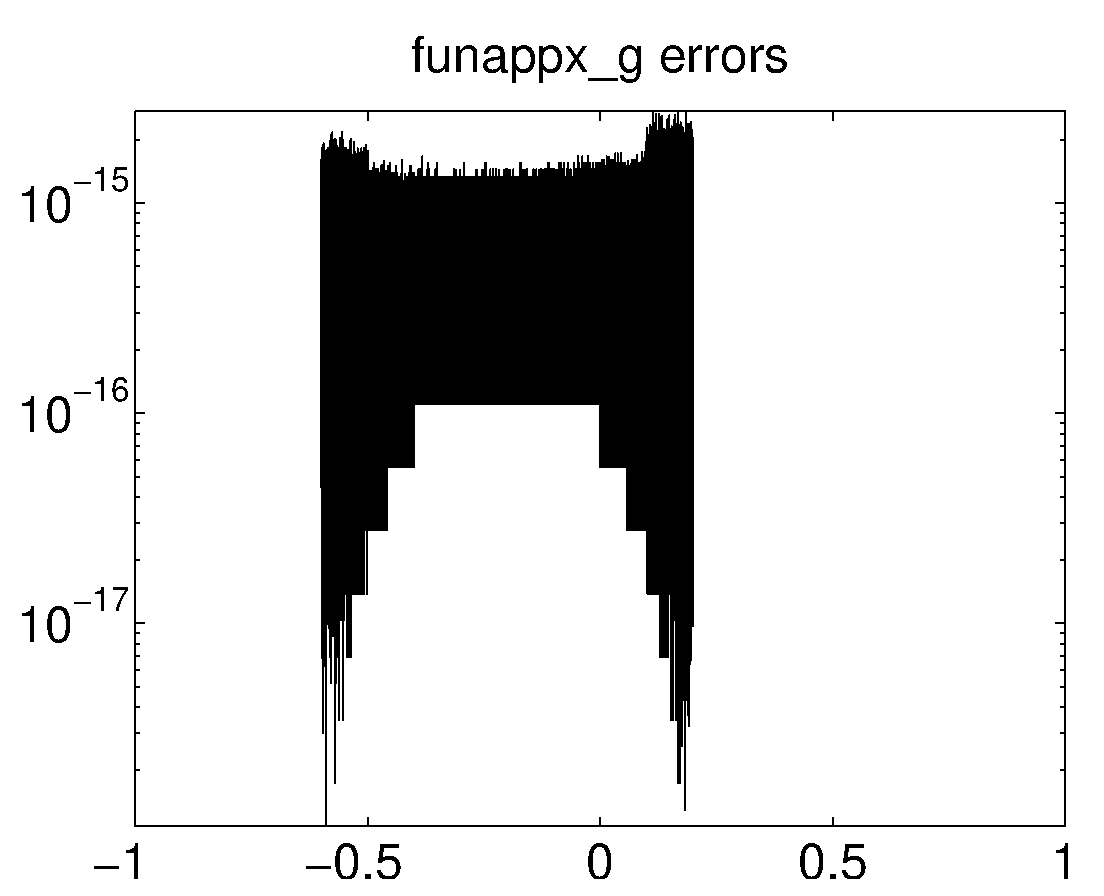
\includegraphics[width=5.7cm]{figure/funappx_g_errors.eps}
\includegraphics[width=5.7cm]{figure/traub_funappx_g_test.eps}
\\ (a) & (b)
\end{tabular}
\caption{(a) The approximation errors for $f_1(x)$ using  Chebfun and  
\funappxg. The blank regions of the graphs correspond to zero errors. 
%This figure is reproducible by \texttt{cf\_chebfun.m}. 
(b) An empirical distribution function of performance ratios based on 1000
simulations for each test function: \funappxg{} time $/$ \funappxglobalg{} time
(blue), \funappxg{} \# of samples $/$ \funappxglobalg{} \# of samples (orange),
\funappxg{} time $/$ Chebfun time (purple), \funappxg{} \# of samples $/$
Chebfun \# of samples (green). This figure is conditionally reproducible by \texttt{cf\_chebfun.m} and
\texttt{traubpaper\_funappx\_g\_test.m} in GAIL.
\label{f3chebfig}} % \label{fig:testfunctions}
\end{figure}

\end{exmp}

\begin{comment}
Our algorithm is readily extensible to the following complex-valued function.
\begin{exmp} This example is taken from MATLAB's documentation for
\texttt{interp1}. Define the complex valued function $v(x) = 5x + x^2 i$ for $x
\in [1,10]$. It is clear that the real part of $v$ is $5x$ and the imaginary
part is $x^2$. We could apply \funappxg to approximate the two parts separately.
However, it is unnecessary.
\end{exmp}
\end{comment}

%% Example 2

\begin{exmp}
In this example, we compare our adaptive algorithms with Chebfun by
simulating the following families of test functions  in addition to $f_1$:
%
\begin{align*}
 g_1(x) &= x^4 \sin(d/x), \qquad
 g_2(x) = 10  x^2 + g_1(x), \qquad x \in [-1, 1].
%\\ f_1(x) &= \begin{cases} \displaystyle
%   \frac{1}{2\delta^2} \Bigl [4 \delta^2 + (x-c)^2 + (x-c-\delta)\abs{x-c-\delta}
%\\ \qquad \qquad
%    - (x-c+\delta)\abs{x-c+\delta} \Bigr ], & \abs{x-c} \le 2\delta,
%\\ 0, & \text{otherwise},
%\end{cases} \\
%\\ g_3(x) & = (x-d)^2,  \qquad
% g_4(x)= d\sin(d\pi x), \qquad
%\\ g_5(x) &= 10\exp\left(-1000(x-d)^2\right), \qquad
% \\ f_4(x)&= \frac{c}{4}\exp(-2x)(c-2\exp(x)(-1 + c\cos(x) - c\sin(x)) \\
%  & \ \ +\exp(2x)(c + 2\cos(x)- 2\sin(x) - c\sin(2x))),
\end{align*}
For $f_1$, we choose $\delta = 0.2$ and $c \sim \cu[0,0.6]$, and for $g_1$, and
$g_2$ we choose and $d \sim \cu[0,2]$. For $d=1$ we obtain $g_i = f_i$ for
$i=1$, and $2$. We set $n_{\text{lo}} = 10$, $n_{\text{hi}} = 1000$, $\fC (h) =
3 \fh/(\fh-h)$ , and $\abstol = 10^{-6}$. Our new algorithm \texttt{funappx\_g},
our old globally adaptive algorithm \texttt{funappxglobal\_g}, and Chebfun are
used to approximate $1000$ random test functions. We switch on the splitting
feature in Chebfun to use piecewise Chebyshev polynomials for approximation if
needed, and override the default tolerance to $10^{-6}$ as well. The
approximation results are summarized in Figure~\ref{f3chebfig}(b) and the upper half of
Table~\ref{tab:localVsGlobalVsChebfun}.

%

%
\begin{table}[bt]
\centering
\caption{Comparison of number of sample points, computational time,  and success
rates of \funappxg (local), \funappxglobalg (global), and Chebfun in upper table;
\funming, \fminbnd, and Chebfun's \texttt{min} in lower table.
%We also report the number of warnings in parentheses issued by the software.
This table can be conditionally reproduced by
\texttt{traubpaper\_funappx\_g\_test.m} and \texttt{traubpaper\_funmin\_g\_test.m}  in GAIL.}
\label{tab:localVsGlobalVsChebfun}
{\footnotesize
\setlength{\tabcolsep}{.15 em} % set table width
		\begin{tabular}{ccrccrccrccrccrccrccrccrccrc}	
		 \hline	
			               &    \multicolumn{9}{c}{\bf Mean Number of Points}   & \multicolumn{9}{c}{\bf Mean Time Used}  & \multicolumn{9}{c}{\bf Success (\%)}
	  \\ \hline  functions &  \multicolumn{3}{c}{local}  &  \multicolumn{3}{c}{global }  &  \multicolumn{3}{c}{Chebfun }  & \multicolumn{3}{c}{local}  &  \multicolumn{3}{c}{global }  &  \multicolumn{3}{c}{Chebfun } & \multicolumn{3}{c}{local}  &  \multicolumn{3}{c}{global }  &  \multicolumn{3}{c}{Chebfun }
\\ \toprule
          $f_1$   &&   2904  &&&   46439   &&&   116    &&&   0.0057   &&&     0.0115    &&&   0.0386 &&&    100   &&&  100   &&&  0
\\        $g_1$   &&   2864  &&&   26265   &&&    43    &&&   0.0080   &&&     0.0092    &&&   0.0083 &&&    100   &&&  100   &&&  3
\\        $g_2$   &&   6911  &&&   97106   &&&    22    &&&   0.0073   &&&     0.0174    &&&   0.0056 &&&    100   &&&  100    &&&  3  	
\\ \hline
%\end{tabular}

%		\begin{tabular}{ccrccrccrccrccrccrccrccrccrc}		
		%	Test      &    \multicolumn{9}{c}{Mean Number of Points}   & \multicolumn{9}{c}{Mean Time Used}  & \multicolumn{9}{c}{Success (\%)}
		% \\ 
			 functions &  \multicolumn{3}{c}{\funming} &  \multicolumn{3}{c}{\fminbnd}  &  \multicolumn{3}{c}{\texttt{min}}
		  &  \multicolumn{3}{c}{\funming}  &  \multicolumn{3}{c}{\fminbnd }  &  \multicolumn{3}{c}{\texttt{min} }  &  \multicolumn{3}{c}{\funming} & \multicolumn{3}{c}{\fminbnd} & \multicolumn{3}{c}{\texttt{min}}
			\\ \toprule
			$-f_1$   &&  274   &&&   8   &&&  116     &&&   0.0022   &&&   0.0010    &&& 0.0469  &&&   100   &&&  100   &&&  14
			\\ $\phantom{-}g_1$   && 230 &&&  22   &&&    43    &&& 0.0020  &&&    0.0012   &&&  0.0109 &&&    100   &&&   27   &&&  60
			\\ $\phantom{-}g_2$   &&  273 &&&   9   &&&   22    &&&  0.0022   &&&   0.0011    &&&  0.0063 &&&    100   &&& 100   &&&  35
			\\ \hline
		\end{tabular}
}
\end{table}
%

Both \funappxg{} and \funappxglobalg{} obtain the correct answer in all cases,
even for $g_1$, which is outside the cone $\cc$. The new locally adapative
algorithm uses fewer samples than the older globally adaptive algorithm. Because it is a higher order algorithm, Chebfun generally used substantially fewer number of samples than
\funappxg, but Chebfun's run time is longer than \funappxg for a
significant proportion of the cases; see Figure~\ref{f3chebfig}(b). However, Chebfun only rarely
approximates the test functions satisfactorily.


\begin{comment}
\begin{table}[tb]
	\centering
	\caption{Comparison of number of sample points, computational time,  and success
		rates of \funming, \fminbnd, and
		Chebfun's \texttt{min}.
		%We also report the number of warnings in parentheses issued by the software.
		This table can be conditionally reproduced by
		\texttt{traubpaper\_funmin\_g\_test.m} in GAIL.}
	\label{tab:funmingVsfminbndVsChebfun}
	{\footnotesize
%		\setlength{\tabcolsep}{.48em} % set table width
%		\begin{tabular}{|c|rrr|rrr|rrrrrr|}
%			\hline
%			Test      &     \multicolumn{3}{c|}{Mean Number of Points} & \multicolumn{3}{c|}{Mean Time Used}  & \multicolumn{6}{|c|}{Success (\%)}
%			\\  family &  \funming  &  \fminbnd    &  \texttt{min}    & \funming     &  \fminbnd  & \texttt{min}   & \multicolumn{2}{r}{\funming} & \multicolumn{2}{r}{\fminbnd} & \multicolumn{2}{r|}{\texttt{min}}
%			\\ \hline
%			-f3   &  274   &   8   &   113    &   0.006   &    0.004    &  0.196  &    100   &  &  100   &   &  12 &
%			\\ \phantom{-}g1   &  230   &  22   &    44    &   0.005   &    0.006    &  0.044  &    100   &  &   24   &   &  54 &
%			\\ \phantom{-}g2   &  273   &   9   &    24    &   0.006   &    0.005    &  0.025  &    100   &  &  100   &   &  34 &
%			\\ \hline
%		\end{tabular}

	\setlength{\tabcolsep}{.3em}
		\begin{tabular}{ccrccrccrccrccrccrccrccrccrc}		
			Test      &    \multicolumn{9}{c}{Mean Number of Points}   & \multicolumn{9}{c}{Mean Time Used}  & \multicolumn{9}{c}{Success (\%)}
			\\  functions &  \multicolumn{3}{c}{\funming} &  \multicolumn{3}{c}{\fminbnd}  &  \multicolumn{3}{c}{\texttt{min}}
		  &  \multicolumn{3}{c}{\funming}  &  \multicolumn{3}{c}{\fminbnd }  &  \multicolumn{3}{c}{\texttt{min} }  &  \multicolumn{3}{c}{\funming} & \multicolumn{3}{c}{\fminbnd} & \multicolumn{3}{c}{\texttt{min}}
			\\ \toprule
			$-f_1$   &&  274   &&&   8   &&&  116     &&&   0.0022   &&&   0.0010    &&& 0.0469  &&&   100   &&&  100   &&&  14
			\\ $\phantom{-}g_1$   && 230 &&&  22   &&&    43    &&& 0.0020  &&&    0.0012   &&&  0.0109 &&&    100   &&&   27   &&&  60
			\\ $\phantom{-}g_2$   &&  273 &&&   9   &&&   22    &&&  0.0022   &&&   0.0011    &&&  0.0063 &&&    100   &&& 100   &&&  35
		\end{tabular}
				
	}
\end{table}
\end{comment}

Similar simulation tests have been run to compare \funming, \fminbnd, and
Chebfun's \texttt{min}. The results are summarized in the lower half of
Table~\ref{tab:localVsGlobalVsChebfun}. Our new \funming{} achieves 100\%
success for all families of test functions with substantially less sampling
points and run time than \funappxg. This is because \funming does not need to
sample densely where the function is not close to its minimum value. Although
\fminbnd uses far fewer function values than \funming, it cannot locate the
global minimum (at the left boundary) for about 70\% of the $g_1$ test cases.
Chebfun's {\tt min} uses fewer points than \funming, but Chebfun is slower and
less accurate than \funming for these test cases.

\end{exmp}


\begin{comment}
\begin{exmp}
In this example, we consider the function $f_4(x) = sin(10 \pi x^4) + x$, which
is increasing oscillating over the interval $[0,2]$. We use \funappxg, \funming,
and \integralg to approximate the function, locate its global minimum, and
estimate its integral with $\abstol = 10^{-8}$. With $1,972,359$ points,
\funappxg can approximate $f_4$ uniformly accurate as shown in
Figure~\ref{f4fig}(a). The true global minimum is $(0.6212340312,
-0.3782149854)$ and the absolute approximation error of \funming using
$n=2,022,621$ points is $(1.4\times 10^{-7}, 4.7\times 10^{-11})$. The integral
$\int_{0}^{2} f_4 (x) dx = 2.145517314$ and the approximation error of
\integralg is $4.7\times10^{-10}$ using $4,965,641$ points.

\begin{figure}[bt]
\centering
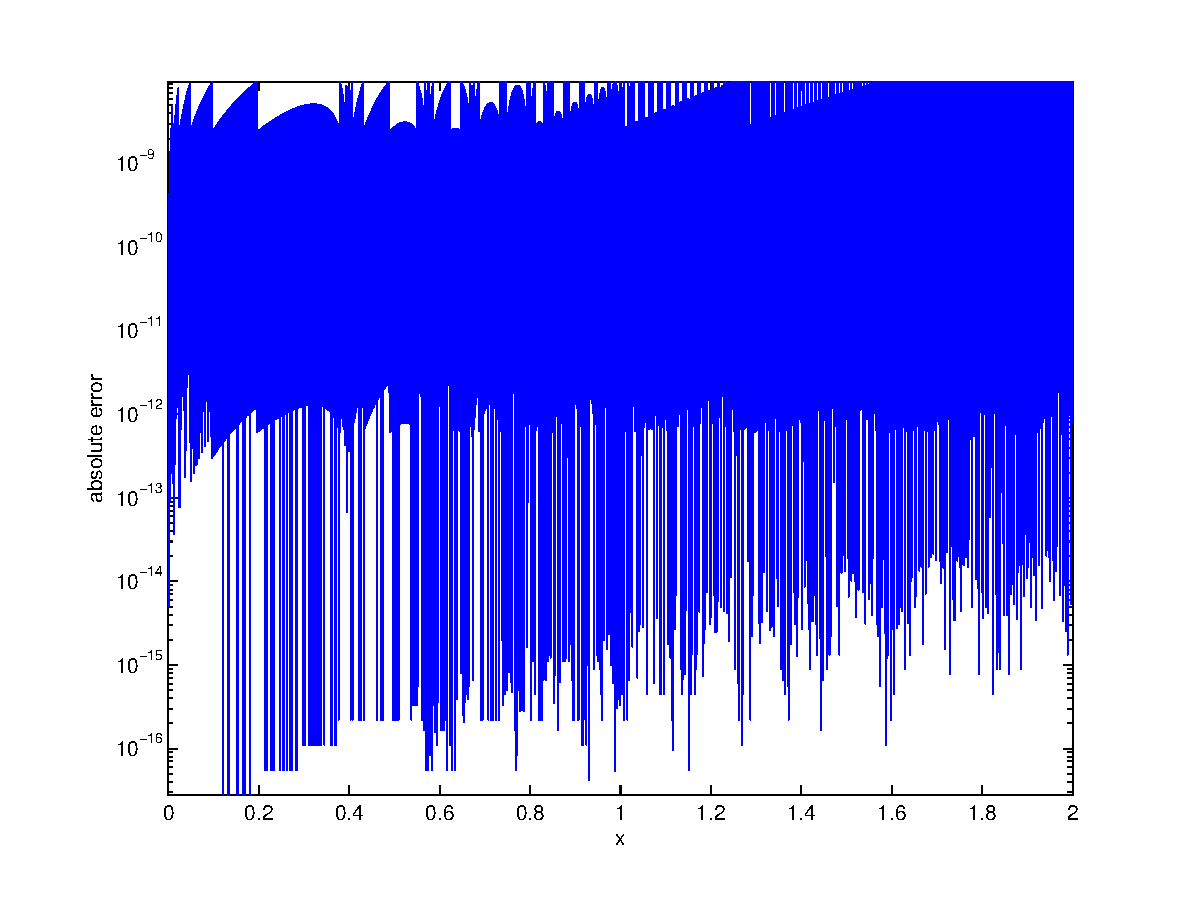
\includegraphics[width=6.2cm]{figure/f4_funappx_error.eps} \hspace{-5ex}
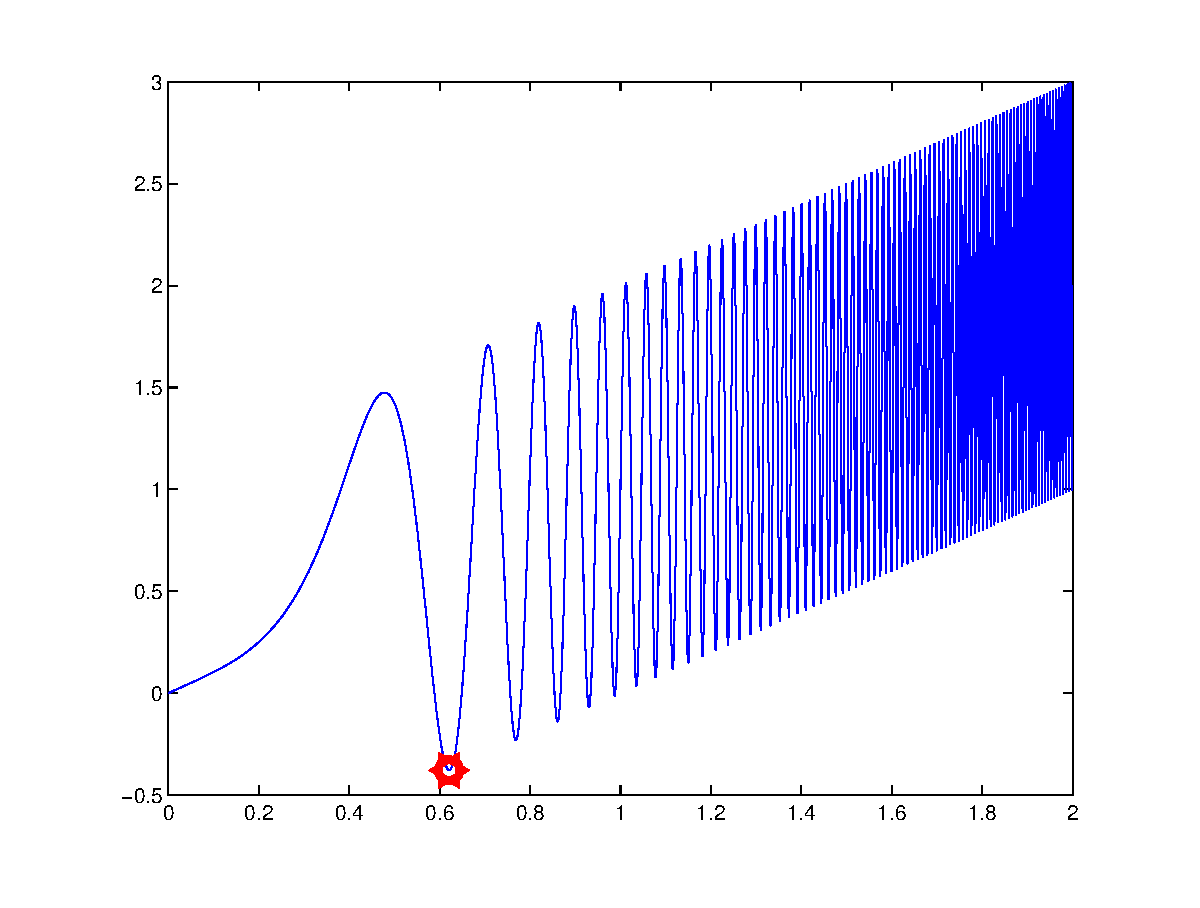
\includegraphics[width=6.2cm]{figure/f4_funmin_g.eps}
\caption{The example $f_4$ with errors of interpolants from \funappxg (left) and
minimum found by \funming (right).}
\label{f4fig}
\end{figure}
\end{exmp}
\end{comment}


\begin{comment}
Our algorithm is readily extensible to the following complex-valued function.
\begin{exmp}
This example is taken from MATLAB's documentation for \texttt{interp1}. Define
the complex valued function $v(x) = 5x + x^2 i$ for $x \in [1,10]$. It is clear
that the real part of $v$ is $5x$ and the imaginary part is $x^2$. We could
apply \funappxg to approximate the two parts separately. However, it is
unnecessary.
\end{exmp}
\end{comment}



%%%%%%%%%%%%%%%%%%%%%%%%%%%%%%%%%%%%%%%%%%%%%%%%%%
\section{Discussion}
%%%%%%%%%%%%%%%%%%%%%%%%%%%%%%%%%%%%%%%%%%%%%%%%%%

Adaptive and automatic algorithms are popular because they require only a
black-box function algorithm and an error tolerance. Such algorithms exist in a
variety of software packages. We have highlighted those found in MATLAB and in
the Chebfun toolbox because they are some of the best. However, as we have shown
by numerical example, these algorithms may fail, and without warning. Moreover,
there is no theory to provide necessary conditions for failure, or equivalently,
sufficient conditions for success.

Our Algorithms $A$ (\funappxg) and $M$ (\funming) are locally adaptive and have
sufficient conditions for success. Although, it may normally be impossible to
verify those conditions in practice, the theory behind these algorithms provide
several advantages: \begin{itemize}
	
\item The conditions defining the cone, $\cc$, have an intuitive explanation as
requiring the second derivative to not change drastically over a small interval.
This intuition can guide the user in setting the parameters defining~$\cc$, if
so desired.
	
\item The norms of $f$ and its derivatives appearing in the computational cost
upper bounds in Theorems \ref{thm:cost} and \ref{thm:Mcost} may not be known.
However, these theorems explain how these norms influence the time required by
Algorithms $A$ and $M$.
	
\item Our Algorithm $A$ has been shown to be asymptotically optimal for the
complexity of the function approximation problem \eqref{appxprob}.
	
\end{itemize}

The minimum horizontal scale of functions in $\cc$ is~$\fh$. The computational
cost of our algorithms is at least $\Order(1/\fh)$, but this is not a
multiplicative factor. Decreasing $\fh$ to make our new algorithms more robust
just increases the minimum number of sample points and may increase the
computational cost mildly through the definition of $\fC$.

There are theorems providing sufficient conditions under which adaption provides
no advantage. Our setting fails to satisfy those conditions because $\cc$ is not
convex. One may average two mildly spiky functions in $\cc$---whose spikes have
opposite signs and partially overlap---to obtain a very spiky function outside
$\cc$.

Moreover, nonadaptive algorithms are unable to solve \eqref{appxprob} or
\eqref{optprob} using a finite number of function values if the set of
interesting functions, $\cc$, is a cone, unless there exist nonadaptive
algorithms that solve these problems exactly. Suppose that $A$ is a nonadaptive
algorithm satisfying \eqref{appxprob} for some cone $\cc$, and that for an error
tolerance $\abstol$, $A$ requires $n$ function values. For any positive, $c$,
define $A^*(f,\abstol) = A(cf,\abstol)/c$ for all $f \in \cc$. Then $\norm{f -
A^*(f,\abstol)} = \norm{cf - A(cf,\abstol)}/c\le \abstol/c$ for all $f \in \cc$
since $cf$ is also in $\cc$. Thus, $A^*$ satisfies \eqref{appxprob} for error
tolerance $\abstol/c$, using the same number of function evaluations as $A$.
Making $c$ arbitrarily large establishes the existence of a nonadaptive
algorithm that solves \eqref{appxprob} exactly.

We recognize that our algorithms do not take advantage of higher orders of
smoothness that the input function may have. We envision the present work as a
stepping stone to developing higher order algorithms. Piecewise interpolants
with higher degrees of smoothness or high degree polynomials, such as those used
in Chebfun, are potential candidates.


\section*{Acknowledgments}

We dedicate this article to the memory of our colleague Joseph F. Traub, who
passed away on August 24, 2015. He was a polymath and an influential figure in
computer science and applied mathematics. He was the founding Editor-in-Chief of
the Journal of Complexity and we are grateful to his tremendous impact and life
long services to our research community.

We thank Greg Fasshauer and the GAIL team for
valuable suggestions and comments. This research was supported in part by grant
NSF-DMS-1522687.



%%%%%%%%%%%%%%%%%%%%%%%%%%%%%%%%%%%%%%%%%%%%%%%%%%
%\section*{References}
%%%%%%%%%%%%%%%%%%%%%%%%%%%%%%%%%%%%%%%%%%%%%%%%%%

\bibliography{FJH23,FJHOwn23}

\end{document}






